\documentclass{article}
\usepackage[T1]{fontenc}
\usepackage[utf8]{inputenc}
\usepackage{lmodern}
\usepackage[a4paper]{geometry}
\usepackage{babel}
\usepackage{amsmath}
\usepackage{xcolor}
\usepackage{graphicx}
\usepackage{amssymb}
\usepackage{algorithm}
\usepackage{algpseudocode}
\usepackage{mathtools}
\usepackage{mathdots}
\usepackage{tikz-cd} 
\usepackage{wrapfig}
\usepackage{float}

% Defines the `mycase` environment.
\newcounter{cases}
\newcounter{subcases}[cases]
\newenvironment{mycase}
{
	\setcounter{cases}{0}
	\setcounter{subcases}{0}
	\newcommand{\case}
	{
		\par\indent\stepcounter{cases}\textbf{Case \thecases.}
	}
	\newcommand{\subcase}
	{
		\par\indent\stepcounter{subcases}\textbf{ \>\>\>\> Subcase (\thesubcases)}
	}
}
{
	\par
}
\renewcommand*\thecases{\arabic{cases}}
\renewcommand*\thesubcases{\alph{subcases}}


\DeclareMathOperator*{\argmin}{argmin}
\DeclareMathOperator*{\pre}{^\bullet}
\usepackage{amsthm}
\usepackage{tikz}
\usetikzlibrary{cd}
\usetikzlibrary{petri,positioning}
\newtheorem{theorem}{Theorem}
\newtheorem{lemma}[theorem]{Lemma}
\newtheorem{remark}{Remark}
\theoremstyle{Definition}
\newtheorem{definition}{Definition}
\theoremstyle{definition}
\newtheorem{example}{Example}
\title{Current Draft\\}
\author{Thomas Chatain, Neha Rino}
\date\today  

\begin{document}
	
	\maketitle 
	
	\begin{abstract}
		The subject of this paper is to study conformance checking for timed models, that is, process models that consider both the sequence of events in a process as well as the timestamps at which each event is recorded. Time-aware process mining is a growing subfield of research, and as tools that seek to discover timing related properties in processes develop, so to does the need for conformance checking techniques that can tackle time constraints and provide insightful quality measures for time-aware process models. In particular, one of the most useful conformance artefacts is the alignment, that is, finding the minimal changes necessary to correct a new observation to conform to a process model.  From alignments, one can derive measures of fitness, precision, and generalisation of a process model, which are crucial to analysing its performance. We develop three metrics by which to compare timed processes, and seek to solve the alignment problem, that is, the problem of calculating the closest trace in the language of a timed model to a particular observed event trace, where each such metric devised provides a new notion of closeness. 
	\end{abstract}
	
	\section{Introduction} 
	
	\subsection{Conformance Checking and Alignments} 
		
	Process mining studies vast systems through their event logs, and seeks to extract meaningful ways to model the underlying patterns or processes that govern the behaviour of the system, sometimes in order to better understand the system, or as is often the case, predict future behaviour \cite{A16}. Once such a process model is obtained, through machine learning or other related techniques, it is natural to ask how one is sure the obtained model is a reasonable approximation of the system’s behaviour at all, especially given the lack of explainability in the blackbox approach ML takes to producing solutions. This is where conformance checking comes into the picture, as it is the art of judging the performance of a process model by comparing its behaviour to the observed behaviour of the system, that is, relating modelled and recorded behaviour of a process to each other, independent of the origin of the model \cite{CDSW18}. Observed behaviour usually comes in the form the traces of an event log, as a sequence of events that often belong to multiple distinct interleaved instances of processes of the system. On the other hand, we have process models, that were either obtained automatically through mining, or were constructed manually, and act a blueprint to describe what the underlying processes of any given system are supposed to look like.  Measures of how well a model reflects reality include fitness, precision, generalisation, and simplicity. We often do not want the system to always precisely generate any and all possible future system behaviour as this will give trivial models accepting for example all execution strings, neither should they simply regurgitate the event log and accept no new system behaviours, a phenomenon known as overfitting. What is often much more useful is a process model that can, up to some small error factor, approximate any reasonable future system behaviour quite closely. This flexible boundary between what is expected and what is possible is precisely what makes a model useful. 
	
	In Aryan Adriansyah's seminal thesis \cite{Adriansyah2014AligningOA} , we obtain the notion of an alignment, that is, the minimal series of corrections needed to transform an observed event trace into the execution of the process model that most closely mimics it.  It is often seen as an execution of the synchronised product of the process model and a \emph{trace model} ie a simple model that captures exactly one event log trace. This gives us a series of edits, usually insertions or deletions, that can transform a model run into the observed run.  For our purposes we will use the term alignment to mean the optimal run of the model that aligns closest to the observation, and how to transform this optimal execution to the observed one will be addressed separately as a matter of distance computation over a set of edit moves. Alignments thereby help pinpoint exactly where inevitable deviations from expected behaviour occur, and the more distant the aligning word of a model is to its observed trace, the worse the model is at reflecting real life behaviour. This can either be used as a tool to help repair the process model to more accurately reflect the observation, or, it can be used to repair the log, or even issue feedback on the behaviour of the underlying system to help it conform to the model better, depending on which components of the operation are the most trustworthy. 
	
	\subsection{Time-aware Processes}
	
		Process models are often formalised using the notion of a Petri net, a standard object used to describe  distributed systems. They both offer a graphical means by which to represent a complex system, and a formal semantics for their execution, which allows one to mathematically analyse the same. They are useful when trying to express dependencies in seemingly parallel parts of the system, the graph structure allowing for branching (i.e. choice), convergence (i.e. synchronisation), and cycles (i.e iteration) in system behaviour. Assuming the event logs are a list of words over a finite alphabet (the set of possible discrete events), the problem of calculating the alignment has been extensively studied \cite{Adriansyah2014AligningOA}, \cite{BCC21}. The notion of distance used on these words used is usually either Hamming distance or Levenshtein's edit distance. Given that Petri net processes already do have certain temporal characteristics, such as a (partial) sense of what happens before and after, and a notion of causal dependency between events, it is natural to want to study explicitly timed systems, that is, systems that not only retain the sequence of events that occur, but the timestamps that show when each event happens. By considering events along with their timestamps when mining processes, observations regarding complex time constraints can be obtained, such as the minimum delay between two events, or the maximum duration the system takes to converge upon a state, or meeting deadlines, all of which are highly relevant in real world applications \cite{Cheikhrouhou2014TheTP}, \cite{Eder1999TimeCI}, \cite{inbook}. In addition, one may want to predict the timestamps of processes \cite{SSA11}. In order to formalise such timed process models, we can use Time Petri nets, that are Petri nets augmented with the ability to record and check the duration it takes to fire a transition once enabled, using which one can impose certain constraints on the relationships between the timestamps of different events. 
		
		So far in the study of the alignment problem for process models, we find one notable gap. The process models concerned often do not consider event timestamps, and constraints imposed upon them. Time-aware process mining seeks to study both what sort of underlying processes govern system behaviour, and what sort of time constraints they can impose on when certain events can occur \cite{RMAW13}, \cite{CRHA20}, \cite{AS21}. The need for such a setting is clear, as specifying and verifying temporal properties, and concrete time constraints regarding the durations of events can provide critical information about a system's behaviour. As time-aware process mining grows popular, new quality measures and conformance checking techniques must be developed that are sensitive to temporal constraints. For this, crucially, one needs to define distance functions that can meaningfully compare and separate different time processes. This paper seeks to provide a framework by which to do the very same.
		
	\subsection{Three Distances, and Algorithms to Align them}
	
		In this paper, we propose three different distance functions over timed words, corresponding to only editing one point in a word at a time (stamp edits), forcing every edit in a word to ripple out and displace all of its causal successors (delay edits), or a combination of the two (mixed edits). The first is essentially Manhattan distance, and hence is extremely practical, and has an efficient algorithm in the case of a structurally restricted class of models (linear causal processes), that is, process models that look like straight lines with no branching or concurrency, but allowing for iteration. For all other types of models, we present an encoding in simplex that solves the problem, albeit with exponential worst-time complexity and good efficiency in practice. The second distance function utilises the structure of the process model to study distances between time processes, and we present a straightforward and efficient algorithm for solving the alignment in this case, but it is limited in its scope of application as it only works if one always knows that every single error will have knock-on effects, such as in event logs that only perceive relative durations but output absolute timestamps. The third is the most versatile, and the most interesting for our purposes. In this setting, edits can either be stamp moves or delay moves, allowing one to choose whether to let an edit stay local or affect the rest of the process, depending on which would be cheaper. We present an algorithm for solving the alignment problem in this setting, but once again only for linearly shaped process models as in the first setting. 
	

	\section{Preliminaries}
	\subsection{Timed Process Models}

	
		We represent events as timed letters, that is of the form $(a,t)$ where $a \in \Sigma$ is the name of the action taken during an event, and $t$ denotes the time at which said action was taken. An event trace is then a sequence of events of the form $\gamma \in (\Sigma \times \mathbb{R}^+)^*$, seen as a timed word.  The timed process model that attempts to capture the behaviour of all observed event traces recorded from the system is represented here as a time Petri net. 
	
	\begin{definition}[Time Petri Net] \label{tpn} A \textit{time Petri net} is a five-tuple $N = (P, T, F, SI, M_0)$, where 
		\begin{enumerate}
			\item $P$ is a set of places 
			
			\item $T$ is a set of transitions 
			
			\item $P \cap T = \emptyset$ 
			
			\item $F \subseteq (P \times T) \cup (T \times P)$ is a flow relation 
			
			\item $SI : T \rightarrow \mathbb{I}$ is the static interval function 
			
			\item$ M_0 \subseteq P$ is the initial marking of $N$
		\end{enumerate}
	\end{definition}
	
	A transition $t$ of a time Petri net is \textit{enabled} at marking $M$ iff $\pre t \subseteq M$. The set of all enabled transitions at a marking $M$ is denoted by \textit{Enabled(M)}. A \textit{state} of a time Petri net $N = (P, T, F, SI, M_0)$ is a pair $S = (M, I)$, where $M$ is a marking of $N$ and $I : Enabled(M) \rightarrow \mathbb{T}$ is called the \textit{clock function}. A transition $t$ may fire from state $S = (M, I)$ after delay $\theta \in \mathbb{T}$ iff $t$ is enabled at $M$, firing $t$ will not result in more than one token at any given place, and updating the clock function with delay $\theta$ will keep $t$'s clock below its latest firing time as determined by the static interval function.  Once it is fired, the marking is updated to $M'$ as in the untimed case (subtracting one token from each preplace, and adding one token to each postplace), and the clock function is updated to increase by $\theta$ for any transition that was enabled at both $M$ and $M'$, set to 0 for any transitions newly enabled by $M'$ that were not enabled at $M$, and left undefined for any that are not currently enabled. 
	
	An important feature of time Petri nets is the notion of urgency, that is, if a transition has been enabled then it must either be disabled (lose some tokens from its preset due to another transition firing) or be fired before the latest firing time lapses. It cannot be allowed to simply \emph{time-out}, i.e, waiting, unfired, throughout the period of time is it capable of firing, and then being disabled just by having the Lft lapse.  
	
	Now we will want to build some vocabulary to help us talk about individual executions of timed words on time Petri nets. These correspond to runs in nondeterministic automata, but in this setting every configuration is a set of token-filled places, so to represent a particular execution we use what we define below as causal processes. 
	
	\begin{definition}[Causal Net] \label{cn}
		A \textit{causal net} $CN = (B, E, G)$ is a finitary, acyclic net where 
		$$\forall b \in B : |b \pre| \leq 1 \wedge | \pre b| \leq 1.$$
	\end{definition}
	
	This is the ground upon which a process of the time Petri net is played. It can be viewed as the original Petri net itself, but every time a place is revisited, it is copied afresh to ensure that the execution only ever moves forward. Hence, multiple elements of $B$ or $E$ map to the same element in $P$ or $T$ respectively, a notion that is expressed via the map $p$ defined below. 
	
	\begin{definition}[Homomorphism] \label{hom}  Let $N = (P, T, F, SI, M_0)$ be a time Petri net and $CN = (B, E, G)$ be a causal net. A mapping $p : B \cup E \rightarrow P \cup T$ is a \textit{homomorphism} if 
		
		\begin{enumerate}
			\item $p(B) \subseteq P$
			\item $p(E) \subseteq T$
			\item $\forall e \in E$ the restriction of $p$ to $\pre e$ is a bijection between $\pre e$ and $\pre p(e)$ and the restriction of $p$ to $e \pre $ is a bijection between $e \pre $ and $p(e) \pre $ and the restriction of $p$ to $Min(CN)$ is a bijection between $Min(CN)$ and $M_0$. 
		\end{enumerate}
	\end{definition}
	
	\begin{definition}[Causal Process]\label{cp} A \textit{causal process} of a TPN is a pair $(CN, p)$ where $CN$ is a causal net and $p$ is a homomorphism from $CN$ to $TPN$. 
	\end{definition}
	
	Using $p$, elements of $CN$ are identified with their corresponding \emph{originals} in the time Petri net, and as a result, any causal process corresponds uniquely to an untimed run on the untimed version of a given time Petri net. 
	
	
	\subsection{Timed Processes}
	
		Now, in order to study \textit{timed} executions, we want to be able add a timing function to the causal process we defined above, thereby allowing us to record when different transitions are taken. The following definitions, properties and theorems in this subsection cover the material developed in Aura and Lilius' article on Time Processes \cite{AL97}. 
	
	\begin{definition}[Timing Function]\label{tau} A \textit{timing function} $\tau : E \rightarrow \mathbb{T}$ is a function from events of a causal process into time values. 
	\end{definition}
	
	Now, given this function, we try to see how the process unfolds. First the initial events, that is, those enabled at $Min(CN)$ happen, and as each event occurs, new events are enabled and disabled. In order to keep track of this, we first define the auxiliary Cut function that represents the effect of having all the events in a subset fire simultaneously (we only use Cut on sets of events that can concurrently fire), as defined below. 
	$$Cut(E') = (E' \pre  \cup Min(NS)) \setminus \pre  E'.$$
	
	Now we can define the  \textit{time of enabling} for a transition $t$ of a TPN in a set of conditions $B'$ of its causal process as $$TOE(B', t) = max(\{\tau(\pre b) | b \in B' \setminus Min(CN) \wedge p(b) \in \pre  t\} \cup \{0\})$$
	
	We must now verify that this timing function does indeed represent a valid execution that obeys all the static interval constraints, as below : 
	
	\begin{definition}[Valid Timing] \label{validt} A timing function $\tau$ is a \textit{valid timing} of the causal process iff 
		$$\forall e \in E : \tau(e) \geq TOE(\pre e, p(e) ) + Eft(p(e))$$ and 
		
		$$\forall e \in E : \forall t \in Enabled (p(C_e)) : \tau(e) \leq TOE(C_e, t) + Lft(t)$$ 
		where $C_e = Cut(Earlier(e))$. 
	\end{definition}

	Here, checking every element of $C_e$ might seem unnecessary but in certain nets, complex dependencies between transitions can cause causally unrelated transitions to force transitions to fire or be disabled, due to urgency. This phenomenon is known as confusion, and hence to guard against this, a timing function must check that it never leaves a section of the process behind, completing the firing or disabling of every event in $Earlier(e)$ before it can reason about the fireability of $e$. 

	\begin{definition}[Time Process] \label{tp} A \textit{time process} of a TPN is a triple $(CN, p, \tau)$ where $\tau$ is a valid timing of $(CN, p)$ which is a causal process of the TPN. 
	\end{definition}
	
	A few last notions here will assist us when we consider a simpler class of time Petri nets, that allow for much easier validity checking. 
	
	\begin{definition}[Extended Free Choice]\label{efc} A time Petri net is \textit{extended free choice} iff for all two transitions $t$ and $t'$, $\pre t \cap \pre t' \neq \emptyset$ implies $\pre t = \pre t'.$
	\end{definition}
	
	This class of time Petri nets ensure that the net is \textit{confusion-free}, that is, causally unrelated events cannot affect the fireability of other events. This means that in order to check for the validity of a timing function, checking all of $C_e$ as before is no longer necessary. 
	
	How do we construct a valid timing function on the fly? Given a partial time process of a TPN, we want to be able to study the effect of firing particular transitions amongst the set of transitions currently enabled. In order to do so, we notice the following class of transitions. 
	
	A transition $t$ is a \textit{choice} at $B' \subseteq B$ iff $B'$ is a co-set that maps injectively to places and $\pre t = p(B')$, and a choice is an \textit{extension} of the process iff $B' \subseteq Cut(E)$. 
	
	These transitions reflect exactly the transitions enabled at a particular moment in the evolution of the process. Either they must be fired or disabled, by the urgency condition. 
	
	Given the above, Aura and Lilius characterise a method by which one can build partial time processes inductively, building forward while maintaining the validity of the timing function, denoted as keeping the process complete with respect to the timing function : 
	
	\begin{definition} A causal process $(CN, p)$ of a time Petri Net where $CN = (B, E, G)$ is said to be \textit{complete} with respect to a timing function $\tau$ iff for every extension transition $t$ of the process, $$\max\{\tau(e)| e \in E\} \leq TOE(Cut(E), t) + Lft(t).$$
	\end{definition}
	
	Now given this, the following theorem due to Aura and Lilius \cite{AL97} holds : 
	
	\begin{theorem}\label{thm35}
		Let $N$ be an extended free choice time Petri net and $(CN, p)$ a causal process of $N$, where $CN = (B, E, G)$. A timing function $\tau$ is valid iff the following criteria hold : 
		
		\begin{enumerate}
			\item$ \forall e \in E :  Eft(p(e)) \leq \tau(e) - TOE(\pre e, p(e))$
			\item $\tau(e) - TOE(\pre e, p(e)) \leq  \min \{Lft(t) | \pre t = \pre p(e)\}$
			\item $(CN, p)$ is complete with respect to $\tau$, i.e, for every extension transition $t$ of the process, $$\max\{\tau(e)| e \in E\} \leq TOE(Cut(E), t) + Lft(t)$$
			
		\end{enumerate}
	\end{theorem}
	
	\subsection{Linear Causal Processes, a small tangent}
	
	We take a moment to discuss a structurally restricted class of processes, that is, causal processes whose graphical structure  is that of a straight line. These reflect the executions of time Petri nets that do not have any branching points ($e \in E : |e \pre | > 1$) and naturally as a consequence, no points of synchrony ($e \in E : |\pre e| > 1$). This loses a significant amount of expressive power, and essentially reflects the executions of automata, allowing for exclusive branching ($p \in P : |p \pre| > 1$) and iteration (that is, cycles in the model) only. On the other hand, studying the language of this restricted class and the alignment problem over it becomes substantially simpler, time processes and their traces are now linear words like one is used to, and $G$ being a total order makes causal dependencies very stable and simple as well, so to begin with, this is a significantly more tractable class of time processes. 
	
	\subsection{The Alignment Problem}
	The alignment problem, given a trace from an event log and a process model, involves finding a valid execution of the process model that is closest to the trace under some metric.
	
	More formally, given a process model $N$ denoted by a Time Petri Net and a timed trace $\sigma$ we wish to find a timed word $\gamma \in \mathcal{L}(N)$ such that $$d(\sigma, \gamma) = \min_{x \in \mathcal{L}(N)} d(\sigma, x)$$ for some distance function $d$ on timed words. 
	
	One might imagine one way to address this case is by the following heuristic : First align the untimed part of the trace with the untimed version of the petri net, and then using the partial order one obtains on the closest untimed trace, proceeding to then try to align the time sequences. While this does neatly separate the problem into the untimed case and a case involving only time sequences, it might not always be very practical. If instead, we decide to view this as a cost minimization problem, given one fixed cost for editing the action names themselves, another fixed cost for editing the time sequences, then the above heuristic is like assigning a significantly higher cost to action edits than time edits, and in some cases this can be an exaggeration. Much like in the untimed case, we may even want to adopt a discounted cost function, ie a cost function that decays as one progresses further in the word, causing earlier errors to be significantly more costly than later ones. 
	
	For the purposes of this paper, we ignore the untimed parts of the words, i.e we assume the underlying causal processes and event labels match, and simply the timing functions on them differ in the words whose distance we wish to measure and minimize. This ensures that we can compare the timing constraints on analogous parts of the process, and hence reason meaningfully about deviances from the model that are purely based on the timing of the process. We try to solve the alignment problem for each of the notions of distance we shall define below.
	
	\section{Some Proposals for Timed Distances} 
	
	Now we come to the problem of deciding how to compare two time sequences, and quantify how close they are to each other. Throughout we assume we are comparing time sequences whose underlying causal processes are the same, in order to meaningfully compare the relationships between their delays. 
	

	\subsection{Edit Moves} 
	
	Much like Levenshtein's edit distance, popularly used in the untimed case of the alignment problem, we view the definition of these distances as an exercise in cost minimisation over the set of all transformations between two words. In order to formalise the same, we need to define what the valid moves of such a transformation could be, as follows : 
	
	We define \textit{moves} as functions that map one timing function over $(CN, p)$ to another. 
	
	We define a \textit{stamp move} as a move that translates the timing function only at a point, ie, that edits a particular element of the timestamp series $\tau$. Calculating $d_t$ between two traces can be viewed as a cost minimization process in aligning the traces using only stamp moves. 
	
	Given a timing function $\gamma : E \to \mathbb{R}$, formally, we define this as : 
	
	$\forall x \in \mathbb{R}, e \in E : stamp(\gamma, x, e) =\gamma' $ where
	
	$$\forall e' \in E : \gamma'(e')  = \begin{cases}
		\gamma(e') + x & e' = e \\
		\gamma(e')& otherwise
	\end{cases}$$
	
	The next type of move we describe is the more novel and interesting \textit{delay move}. By formulating this type of edit move, we sought to leverage the structure of the process model itself, by reflecting the causal relationships the pre-order $G$ causes. If an event is $G$-reachable from another, that means the first event is strictly in the causal history of the second. One can conceive of situations where changing the timestamp of such a causal predecessor has consequences for all of its causal descendents, while leaving any causally unrelated (i.e, non-$G$-reachable) events undisturbed. This is the motivation behind a delay edit. A stamp move is purely local, such that when a stamp edit occurs at $e$ its immediate successor events shift their relationship with $e$, thereby ensuring that the change in $e$'s timestamp does not derail the rest of the system. On the other hand, any delay move at $e$ will preserve relative relations in the future, at the cost of shifting the timestamp of every causal descendent of $e$ by the same amount. Alternatively, this formulation of a move can be seen as ensuring one need not pay multiple costs for translating an entire causally linked branch of the process by a certain amount, instead editing (and paying) just once, judiciously early on, and reaping its rewards later without cost. 
	
	So, we define a \textit{delay move} as a move that translates the timing function at a point and all of its $G$-successors. Calculating $d_\theta$ between two traces can be viewed as a cost minimization process in aligning the traces using only delay moves. 
	
	Given a timing function $\gamma : E \to \mathbb{R}^n$, we define a delay move applied to it as follows : 
	
	$\forall x \in \mathbb{R}, e \in E : delay(\gamma, x, e) = \gamma'$ where 
	
	$$\forall e' \in E : \gamma'(e') = \begin{cases}
		\gamma(e') + x & e' \geq_G e \\
		\gamma(e')& otherwise
	\end{cases}$$

	It will often be convenient to consider the following representation when speaking about delay moves, and so we define a way by which to view a timed word not in terms of its absolute timestamps, but by the delays between relevant timestamps. 
	
	Given a causal process $(CN, p)$ over $N$, where $CN = (B, E, G)$, and a (not necessarily valid) timing function $\tau : E \to \mathbb{R}^+$, we first define the auxiliary \textit{flow} function $f_{\tau} : E \to \mathbb{R}^+$ such that 

	$$f_{\tau}(e) = \begin{cases} 
	\tau(e) & \pre \pre e = \emptyset\\
	\tau(e) - \tau(e') &e' \in   \pre \pre e, \tau(e') = \max\limits_{e'' \in \pre \pre e} {\{\tau(e'')\}} \cup \{0\}\\
\end{cases}
$$
	
	Now a delay move is quite clearly a simple local edit of the flow function $f_\tau$ as defined above. 
	
	We will also define a third kind of move, although really it is simply convenient notation for a common combination of the previous two rather than a new mechanism of transformation. We define \textit{mixed moves}, that denote doing a stamp move and a delay move at the same position in the word. Let $Moves(CN, p) = \{(s, d, e) | s, d \in \mathbb{R}, e \in E\}$ be the set of possible mixed moves over any trace with underlying causal process $(CN, p)$. We define their effect as follows : $$(s, d, e)(\gamma) = stamp(delay(\gamma, d, e), s, e)$$
	
	Given any move $m \in Moves(CN, p)$ we define the function $cost : Moves(CN, p) \to \mathbb{R}^+$ that returns the cost of the move.  The cost of a mixed move $(s, d, e)$ is the sum of the cost of the stamp and delay moves it's made up of, $|s| + |d|$.
	
	We say a sequence of moves $m_1m_2\dots m_n = m \in Moves(CN, p)^*$ \textit{aligns} $\tau_1$ to $\tau_2$ if $$m(\tau_1) = m_n(\dots (m_2(m_1(\tau_1))\dots) = \tau_2$$
	
	We use the notation $m|_{i}$ to denote the $i$-length prefix of $m$, that is, $m_1 \circ m_2 \circ \dots m_i$. 
	
	For a language $\mathcal{L}(N)$, the restriction of the language to its $i$-length prefixes is denoted by $\mathcal{L}^i(N)$.
	
	Now with all this notation, we consider three different settings with which we can define distances. 
	

	\subsection{Stamp only distance}
	
		This represents the case where only stamp moves can be used to transform a word into another. This is seen to be equivalent to the \textit{Manhattan distance} or \textit{taxicab distance} between two points of $\mathbb{R}^n$, say $\mathbf{t} = (t_1, t_2, \dots t_n) $ and $\mathbf{s} = (s_1, s_2, \dots s_n)$, defined as $$d_t(\mathbf{t}, \mathbf{s}) = \sum_{i = 1}^{n} |t_i - s_i|$$
	
	The way we see this is as follows. Given a causal process $CN = (B, E, G)$ and two timing functions (not necessarily constituting valid timings) $\tau_1, \tau_2$, let $$d_t(\tau_1, \tau_2) = \sum_{e \in E} |\tau_1(e) - \tau_2(e)|$$
	This is both achievable by stamp only moves by doing the corresponding $\tau_1(e) - \tau_2(e)$ stamp move to the second word, and is the least cost any such stamp only path can take as Manhattan distance obeys the triangle inequality, and every stamp move results in a word at exactly the same Manhattan distance from its predecessor as the cost of said stamp move. 
	
	\begin{example}\label{stamptoy}
		Consider the following example : 
		
		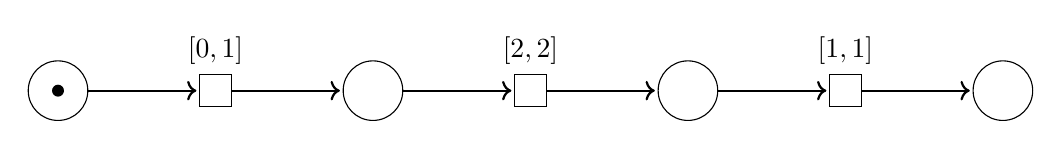
\begin{tikzpicture}
			
			\node[place, tokens = 1] (p1) at (0,0) {}; 
			
			\node[transition, label ={ $[0,1]$}] (t1) at (2,0) {}; 
			
			\node[place] (p2) at (4,0) {}; 
			
			\node[transition, label ={ $[2,2]$}] (t2) at (6,0) {}; 
			
			\node[place] (p3) at (8,0) {}; 
			
			\node[transition, label ={ $[1,1]$}] (t3) at (10,0) {}; 
			
			\node[place] (p4) at (12,0) {}; 
			
			\draw[thick] (p1) edge[post] (t1)
			(t1) edge[post] (p2)
			(p2) edge[post] (t2)
			(t2) edge[post] (p3)
			(p3) edge[post] (t3)
			(t3) edge[post] (p4);
			
		\end{tikzpicture}
		
		Now for this $N$, let the observed trace $\sigma = (0,3,4) \not \in \mathcal{L}(N)$. 
		
		The best $d_t$ alignment for the example in the diagram below is $\gamma_t = (1,3,4)$ because
		
		$$d_t(\gamma_t, \sigma) = 1 \leq d_t((x, x+2, x+3), \sigma) = |x| + 2|x-1|, \forall x \in [0, 1]$$
	\end{example}	
	
	
	\subsection{Delay only distance}
	
		We now look at a possible distance function for time sequences obtained by minimising the cost over paths that are only allowed to perform delay moves. This distance function actually takes advantage of the structure of the process model $N$, a Time Petri Net, and we call it $d_\theta$. Aside from the definition based on moves, we can define $d_\theta$ directly using the flow function previously defined, as follows : 
	$$d_\theta(\tau_1, \tau_2) = \sum_{e \in E}|f_{\tau_1}(e) - f_{\tau_2}(e)|$$
	
	Note that $e'$ as defined here is the latest causal predecessor of $e$, that is, it is the firing of $e'$ that enabled $e$. Hence, $f_\tau$ as defined produces exactly the time durations that the guards of each transition in the model checks, ie the clock function values during the run. 
	
	This distance can be seen to be identical to the distance we obtain by minimising on delay only moves by noting that delay moves on a trace $\tau$ are the same as stamp moves on $f_\tau$, and using the same argument as in the previous section. 
	
	As defined, we see that if a word is in the language of the model, then its $f$ function maps events to values that lie within the constraint that the event's corresponding transition demands, that is, it is perfectly aligned with the model with distance 0. This condition is unfortunately not sufficient though, due to urgency concerns, but it is quite close to the exact condition necessary for a word to be in the language of a time Petri net. 
	
	Also note that given the underlying causal process and the resulting $f_\tau$, we can reconstruct $\tau$ quite straightforwardly as $$\forall e \in E : \tau(e) = \sum_{e' \leq_G e} f_\tau(e')$$
	

	\begin{example}
		Studying the model and observed trace seen in Example \ref{stamptoy}, but in the delay only setting, we see that since $\mathcal{L}(N) = \{ (x, x+2, x+3) | \forall x \in [0, 1] \}$, the best $d_\theta$ alignment for the above trace and model pair is $\gamma_\theta = (0,2,3)$ because
		
		$$d_\theta(\gamma_\theta, \sigma) = 1 \leq d_\theta((x, x+2, x+3), \sigma) = |x| + 1, \forall x \in [0, 1]$$
	\end{example}
	
	
	\subsection{Mixed moves distance}
	
		Finally we define one more possible distance function, combining the previous two concepts. Here, we allow for either editing absolute timestamps or relative time durations via delays, that is, we allow the use of either type of move. 
	
	Given two timing functions $\tau_1, \tau_2$ and their underlying causal process $(CN, p)$, we define $d_N(\tau_1, \tau_2)$ to be the minimum total cost over all possible sequences of moves that align $\tau_1$ to $\tau_2$. 
	
	Computing this distance is no longer straightforward the way it was for the first two settings. As an example, consider the following : 

	\begin{example}\label{oldmodelmixex}
		Now, coming back to the model and observed trace we studied in Example \ref{stamptoy}, but now in the mixed setting. Once again, we note that any word in the language would be of the form $(x, x+2, x+3)$ with $x \in [0, 1]$. 
		
		Now intuitively, when dealing with linear models where the ripple effect of a delay is always predictably to the right irrespective of the values of the timestamps, moves can be applied in any order, so we can assume a minimum cost move is chronological. So our first move will have to incur a minimum cost of $|x| = x$ as we try to align $(0,3,4)$ to our model. Now, if any part of this initial move was a delay, we would push the second component even further away from $x+2$ than it already was, and if any of the delay were negative, then the mixed move seems counterproductive at the first component as the delay and stamp moves work against each other, so let us say the first move was pure stamp. Now we move on to move two, which will again incur a minimum cost of $|1-x| = 1-x$. Now, if the stamp part of this move were positive, it would leave the third component further off from the goal $x+3$ than if all of the move was delay, and so a pure delay move seems best here. Hence, the least cost alignment is $(x, 0, 1)(0, 1-x, 2)$, with total cost 1. 
		
		All the intuitive reasoning given above will be justified in subsequent sections, and in fact distance 1 is the best we can do here even in the mixed case. Hence the aligning words here constitute the whole language $\mathcal{L}(N)$ as they are all at distance 1 from the observed trace in this setting. 
	\end{example}
	
	
\begin{example}\label{mixedmoveex}
	Consider the same underlying linear model, and a new observed trace. 
	
	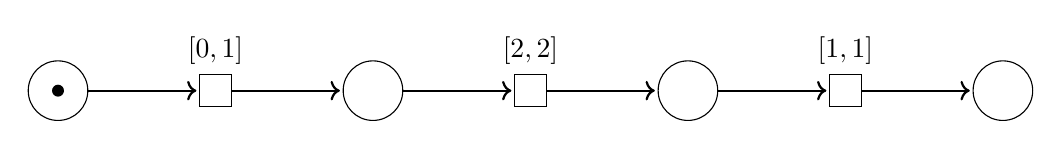
\begin{tikzpicture}
		
		\node[place, tokens = 1] (p1) at (0,0) {}; 
		
		\node[transition, label ={ $[0,1]$}] (t1) at (2,0) {}; 
		
		\node[place] (p2) at (4,0) {}; 
		
		\node[transition, label ={ $[2,2]$}] (t2) at (6,0) {}; 
		
		\node[place] (p3) at (8,0) {}; 
		
		\node[transition, label ={ $[1,1]$}] (t3) at (10,0) {}; 
		
		\node[place] (p4) at (12,0) {}; 
		
		\draw[thick] (p1) edge[post] (t1)
		(t1) edge[post] (p2)
		(p2) edge[post] (t2)
		(t2) edge[post] (p3)
		(p3) edge[post] (t3)
		(t3) edge[post] (p4);
		
	\end{tikzpicture}
	
	Now for this $N$, let the observed trace $\sigma = (3, 4, 5) \not \in \mathcal{L}(N)$. 
	
	The best $d_t$ alignment for the example in the diagram below is $\gamma = (1,3,4)$ with minimum cost $d_t(\sigma, \gamma) = 4$. 
	
	The best $d_t=\theta$ alignment for the example in the diagram below is also $\gamma = (1,3,4)$, but this time with minimum cost $d_\theta(\sigma, \gamma) = 3$. 
		
	And lastly, the best $d_N$ alignment for the example in the diagram below is also $\gamma = (1,3,4)$, the sequence of moves being simply one mixed move at the start, $m = (-1, -1, 1)$, and now with minimum cost $d_N(\sigma, \gamma) = 2 < \min \{d_t(\sigma, \gamma), d_\theta(\sigma, \gamma)\}$. 
\end{example}

	\section{Delays Only }

	The delay only distance, $d_\theta$, is built so as to allow local edits that do not affect global membership in the language of the time Petri net, as both the time Petri net and delay edits concern themselves only with the duration of time elapsed between a transition's enabling and its firing. This relationship is especially clear in extended free choice time Petri nets, where the only events that determine the fireability of an event are its causal history and events with the exact same preset, which would naturally disable it by firing. Hence, we present the following algorithm, which minimizes the delay cost at each transition locally, while still overall ensuring membership in the language of the model. 
	
		\begin{algorithm}
		\caption{Naive $d_\theta$ Algorithm}
		\label{DelayAlgo}
		\begin{algorithmic}[1]
			
			\State \textbf{Input : }  $N$, $CN = (B, E, G), p$, $\sigma : E \to \mathbb{R}^+$
			\State \textbf{Output : }  $\gamma : E \to \mathbb{R}^+$ such that $(CN, p, \gamma)$ is a valid time process of $N$ and $d_\theta(\gamma, \sigma)  \leq  {d_\theta(x, \sigma)}$ for all $x$ such that $(CN, p, x)$ is a valid time process of $N$\\
			
			\State $Curr = Min(CN)$
			\State $Enabled = \{t | \pre t \subseteq p(Curr)\}$
			\State $FD = \{(t, eft, l, toe) | t \in Enabled, eft = Eft(t), toe = 0, l = \min_{\pre t' = \pre t}{Lft(t')}\}$
			\State $Soon = \{(t, eft, l, toe) \in FD | l+toe \textrm{ is minimal in } FD\}$
			
			\While{ $E \neq \emptyset$} 
			\If {$\pi_1(Soon) \cap p(E) = \emptyset$} 
			\State REJECT : invalid causal process 
			\State \textbf{return} None  
			\Else : 
			\State Pick $(t, eft, l, toe) \in Soon, t \in p(E)$ 
			\State $E \gets E \setminus\{e | p(e) = t\}$
			\State $e \gets p^{-1}(t)$
			\State $Curr \gets \{Curr \setminus \{\pre e\}\} \cup \{e \pre\} $
			\State $f_{\gamma}(e) = \argmin_{x in [eft, l]}|x - f_{\sigma}(e)|$
			
			\ForAll{$t' \in T \wedge \pre t' = \pre t$} 
			\State $Enabled \gets Enabled \setminus\{t'\}$
			\State $FD \gets FD \setminus\{(t', e', l', toe')\}$
			\EndFor
			
			\ForAll{$t' \in T \wedge t' \pre = t \pre$}
			\State $Enabled \gets Enabled \cup \{t'\}$
			\State $eft' \gets Eft(t')$
			\State $l' \gets \min_{\pre t'' = \pre t'}{Lft(t'')}$
			\State $toe' \gets toe + f_\gamma(e)$
			\State $FD \gets FD \cup \{(t', eft', l', toe')\}$
			\EndFor
			\State $Soon = \{(t, eft, l, toe) \in FD | l+toe \textrm{ is minimal in } FD\}$
			\EndIf
			\EndWhile
			\State \textbf{return } $\gamma$
			
		\end{algorithmic}
	\end{algorithm}
	
	
	\begin{theorem}\label{DelayAlgoCorr} Algorithm \ref{DelayAlgo} is correct on extended free choice time petri nets, that is, its result $\gamma$ has the properties : 
		\begin{enumerate}
			\item $(CN, p, \gamma$ is a valid time process of $N$. 
			\item $d_\theta(\gamma, \sigma)  \leq  {d_\theta(x, \sigma)}$ for all $x$ such that $(CN, p, x)$ is a valid time process of $N$. 
		\end{enumerate}
	\end{theorem}
	
	
	\begin{proof}
		By theorem \ref{thm35} proved in Aura and Lilius' article \cite{AL97}, we know that in order to ensure that this is a valid time process, we need only ensure three inequalities hold as the time process $\gamma$ evolves. 
		
		\begin{enumerate}
			\item$ \forall e \in E :  Eft(p(e)) \leq \gamma(e) - TOE(\pre e, p(e))$
			
			By definition $f_\gamma(e) = \gamma(e) - TOE(\pre e, p(e))$, and by line 6 of the algorithm the variable $eft$ is correctly initialised to store $Eft(p(e))$, and line 17 ensures the above inequality holds. 
			
			\item $\gamma(e) - TOE(\pre e, p(e)) \leq  \min \{Lft(t) | \pre t = \pre p(e)\}$
			
			In similar vein, line 6 also ensures that $l$ is initialised precisely to store $\min \{Lft(t) | \pre t = \pre p(e)\}$, and line 17 again enforces the left hand side to be less than $l$. 
			
			\item $(CN, p)$ is complete with respect to $\gamma$, i.e, for every extension transition $t$ of the process, $$\max\{\gamma(e)| e \in E\} \leq TOE(Cut(E), t) + Lft(t)$$
			
			At every point when assigning a timestamp to an event, it is ensured that it belongs to $Soon$, a set defined to contain only those enabled events that have the least value of $l + toe$, or, $TOE(Cut(E), p(e)) + Lft(p(e))$. This ensures that whenever an event $e$ is assigned a timestamp $\gamma(e)$, for all extension transitions $t$  (which must either be causal descendents of $e$ or already enabled when $e$ was picked, thereby being in $Enabled$, by extended free choice) we know that $\gamma(e) \leq TOE(Cut(E), p(e)) + Lft(p(e)) \leq TOE(Cut(E), t) + Lft(t)$. 
			
			Hence, $(CN, p, \gamma)$ is a valid time process of $N$. 
			
		\end{enumerate}
	
	As for its optimality, we see that any other valid time process would have to obey the same inequalities, in particular for another valid timing function $\gamma'$ it would have to obey $$f_{\gamma'}(e) \in [Eft(p(e)), \min_{\pre t' = \pre p(e)}{Lft(t')}] = [a,b]$$ and hence at any event $e$ where $\gamma$ differs from $\gamma'$ it would have lower than or equal cost for that event as $$f_\gamma(e) = \argmin_{x \in [a, b]} |f_\sigma(e) - x|$$
	
	Hence, the algorithm is correct. 
		\end{proof}
	
	\begin{remark} Note that Algorithm \ref{DelayAlgo} runs through the events of the causal process $E$ exactly once, and each time runs through the set of currently enabled transitions, and the total set of transitions, and hence its time complexity is linear in the size of the input $|CN|$, and the size of the transition set, i.e, $O(|E||T|)$. 
	\end{remark}
	
	
	\section{Stamp Only} 
	\subsection{Linear Case} 

We are given a process model $N$, an observed trace $\sigma$, and its underlying linear causal process $CN = (B, E, G)$ with homomorphism $p$ for the untimed run of $\sigma$ on $N$. Suppose we tried to express the cost of aligning a prefix of $\sigma$ to some timing function $\tau$ on the truncation of the linear causal process up to the $i$th transition, call it $cost$. 

$$cost(\tau|_i) = \sum_{j = 1}^{i} |\tau_j - \sigma_j|$$

Now, note the following equation holds for the $(i+1)$th static interval constraint $[a, b]$ : 

$$\min_{\tau|_{i+1} \in \mathcal{L}^{i+1}(N)}cost(\tau|_{i+1}) = \min_{\tau_{i+1} - \tau_i\in [a, b]} (|\tau_{i+1} - \sigma_{i+1}| + \min_{\tau|_i \in \mathcal{L}^i(N) }cost(\tau|_i))$$

This suggests that the minimal cost of aligning prefixes $\sigma$ to prefixes of the model can be recursively calculated as a function of the value of the last timestamp in the alignment of a given prefix. $$g_i(d) = \min_{\tau|_i \in \mathcal{L}^i(N) \wedge \tau_i = d} cost(\tau|_i)$$

Now, the previous equation can be expressed in terms of the $g$ functions as follows : 

$$g_{i+1}(d) = |d - \sigma_{i+1}| + \min_{d-d' \in [a,b]} g_i(d')$$

If we can calculate the family of functions $\forall i \leq n : g_i$ efficiently, then the minimal cost for aligning $\sigma$ to $N$ is simply $$\min_{d} g_n(d)$$


\begin{example}
	
	
	We take a moment to look at an example of the computation of this family of functions we proposed by considering the following $d_t$-alignment problem : 
	
	We first have the process model $N$ : 
	\\
	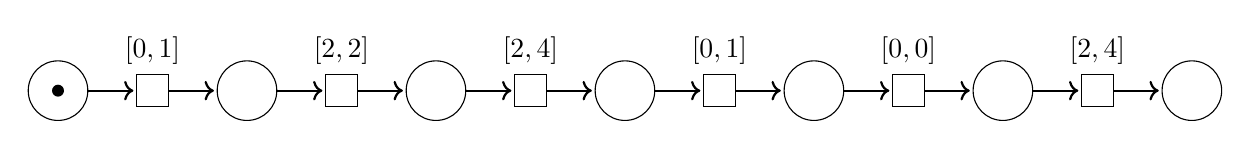
\begin{tikzpicture}
		
		\node[place, tokens = 1] (p1) at (0,0) {}; 
		
		\node[transition, label ={ $[0,1]$}] (t1) at (1.2,0) {}; 
		
		\node[place] (p2) at (2.4,0) {}; 
		
		\node[transition, label ={ $[2,2]$}] (t2) at (3.6,0) {}; 
		
		\node[place] (p3) at (4.8,0) {}; 
		
		\node[transition, label ={ $[2,4]$}] (t3) at (6,0) {}; 
		
		\node[place] (p4) at (7.2,0) {}; 
		
		\node[transition, label ={ $[0,1]$}] (t4) at (8.4,0) {}; 
		
		\node[place] (p5) at (9.6,0) {}; 
		
		\node[transition, label ={ $[0,0]$}] (t5) at (10.8,0) {}; 
		
		\node[place] (p6) at (12,0) {}; 
		
		\node[transition, label ={ $[2,4]$}] (t6) at (13.2,0) {}; 
		
		\node[place] (p7) at (14.4,0) {}; 
		
		\draw[thick] (p1) edge[post] (t1)
		(t1) edge[post] (p2)
		(p2) edge[post] (t2)
		(t2) edge[post] (p3)
		(p3) edge[post] (t3)
		(t3) edge[post] (p4)
		(p4) edge[post] (t4)
		(t4) edge[post] (p5)
		(p5) edge[post] (t5)
		(t5) edge[post] (p6)
		(p6) edge[post] (t6)
		(t6) edge[post] (p7);
		
	\end{tikzpicture}
	\\
	The observed trace is $$\sigma = (1,2,4,6,6,8)$$
	%%
	
	\begin{figure}
		\centering 
		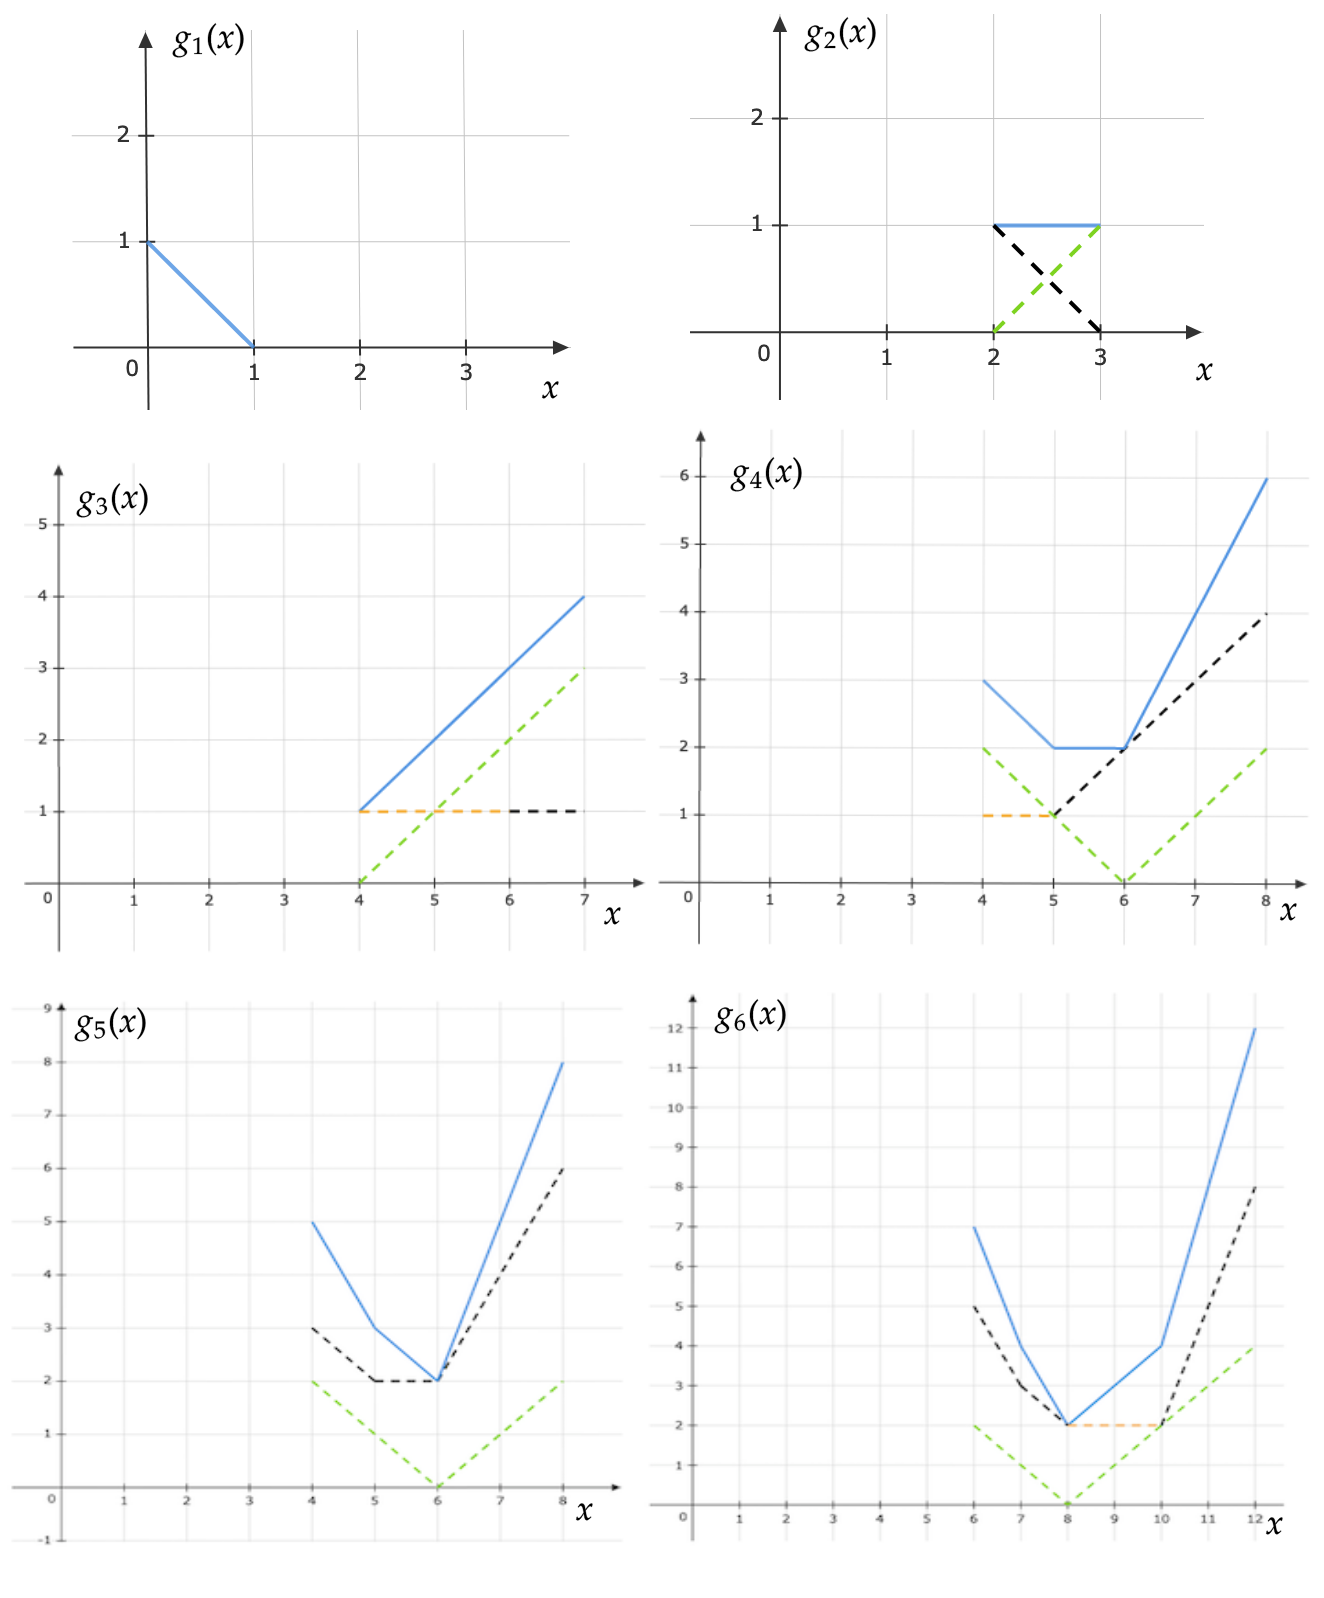
\includegraphics[width = \textwidth]{stampgraph.png}
		\caption{Visual representation of the algorithm on the example above}
	\end{figure}

	Now, we begin to compute the family of functions $g_i$, starting with $g_1(x) = |1-x|$ in the domain $[0,1]$.
	
	Now, utilising the recursion, we try to compute $g_2$.  
	
	The new domain is $[2,3]$, a simple translation of the previous one because the guard on the second transition is the point $[2,2]$. Now, we want the sum of both $|x-2|$ and $\min_{x' - x \in [2,2]}g_1(x')$. The first of these functions, that is the contribution of the last timestamp to the error, is pictured in figure 1 in green dashed lines. The second component is pictured in black dashed lines. In this case, the non-green dashed component is simply a translation of $g_1$, as $\min_{x' - x \in [2,2]}g_1(x') = g_1 - 2$. 
	
	Now, let us construct $g_3$ similarly, by summing the contribution of the last timestamp, $|x - 4|$, to  $\min_{x' - x \in [2,4]}g_2(x')$. We now have an orange segment in the second component! This is used to demarcate any additional segments not present in the previous $g$-function (if any). We see the effect of the $\min$ operation is simply to attach a segment with the same length as the $i$th static interval constraint, at the lowest point of $g_{i-1}$. Now we begin to see a simple way to construct these graphs visually : The next black graph is a translation of the previous blue one, with an orange line segment or the same length as the next static interval constraint inserted at the lowest point, and the next green graph is simply $|x-\sigma_i|$ in the new domain, and summing these two gives the next blue graph. Even summation is simpler than it looks, as these are all piecewise linear graphs, so you can simply increment the slopes of all the segments of the black-orange curve by one if they're to the right of $\sigma_i$, and by minus one if they're to the left, and translate the height up as needed. Clearly the orange, black and green segments of the next graph are obtained like this, and $g_4$ is their sum. 
	
	The procedure for constructing $g_5$ and $g_6$ are identical, and now finally we see that the minimum cost of $2$ is achieved in $g_6$ by setting the last timestamp to $8$. Now, we know the contribution of the $8$ to the error is zero, so this means we can deduce the corresponding value in $g_5$ must have been $2$ as well, achieved when the fifth timestamp was set to $6$. Now $6$ gives a contribution of $0$ again to the error, letting us look at the preimage of $2$ once again on $g_4$, and so on. We can backtrack in this manner to build an optimal alignment, such as in this case, $(1,3,5,6,6,8)$. 
\end{example}


With this context, we present the following algorithm that progressively calculates the graphs of $g_i$ each round, and claim it is both correct and efficient : 

\begin{algorithm}
	\caption{$d_t$ Algorithm}
	\label{StampAlgo}
	\begin{algorithmic}
		
		\State \textbf{Input : }  $\sigma$, a list of static interval constraints for the linear model $SI$
		\State \textbf{Output : }  $cost = \min_{x \in \mathcal{L}(N)}{d_t(x, \sigma)}$, $\gamma \in \mathcal{L}(N)$ such that $d_t(\gamma, \sigma) = cost$\\
		
		\State \textbf{Object :} $graph = \{(left, slope, right) | graph[i].left = graph[i-1].right\}$
		
		\Procedure{StampOnlyAlgo}{$\sigma, SI$}
		\State Initialise System 
		\State $a \gets \pi_1(SI[0])$
		\State $b \gets \pi_2(SI[0])$		
		\State $graph \gets \{(a, 0, b)\}$
		\State \textsc{graphAddMod}($graph, \sigma[0]$)
		\State $graphlist \gets \{graph\}$
		\State $i \gets 1$
		\State $cost \gets |a - \sigma[0]|$
		
		\While{$i < |sigma|$}
		\State $a \gets \pi_1(SI[i])$
		\State $b \gets \pi_2(SI[i])$		
		\State \textsc{graphMin}($graph, a, b$)
		\State \textsc{graphAddMod}($graph, \sigma[i]$)
		\State $graphlist.append(graph)$
		\State $cost \gets cost + |a - \sigma[i]|$
		\EndWhile
		
		\State $i \gets 0$ 
		\State $s \gets graph[0].slope$
		
		\While{$graph[i].slope < 0$}
		\State $s \gets graph[i].slope$ 
		\State $cost \gets cost + s * (graph[i].right - graph[i].left)$
		\State $i \gets i + 1$
		\EndWhile
		
		\State $\gamma \gets \textsc{backTrack}(\sigma, graphlist, cost)$
		\State \textbf{Return : } $cost, \gamma$
		\EndProcedure
		
	\end{algorithmic}
\end{algorithm}



\begin{algorithm}
	\caption{$g_i(d) \to g_i(d) + |d-x|$}
	\label{AuxFunc1}
	\begin{algorithmic}
		
		\Procedure{graphAddMod}{graph, x} 
		\State $l \gets graph[0].left$
		\State $r \gets graph[-1].right$ 
		\State $i = 0$
		
		\While{$i < |graph|$}
		
		\If{$graph[i].right \leq x$} 
		\State $graph[i].slope \gets graph[i].slope -1$
		
		\ElsIf{$graph[i].left < x \wedge graph[i].right > x$}
		\State $slope \gets graph[i].slope$
		\State $high \gets graph[i].right$
		\State $graph.insert(i+1, (x, slope, high))$
		\State $graph[i].right \gets x$
		\State $graph[i].slope \gets slope - 1$
		
		\Else
		\State $graph[i].slope \gets graph[i].slope + 1$
		\EndIf
		
		\State $i \gets i +1$
		\EndWhile
		\EndProcedure
		
	\end{algorithmic}
\end{algorithm}



\begin{algorithm}
	\caption{$g_i(d) \to \min_{d - d' \in [a,b]}{g_i(d')} $}
	\label{AuxFunc2}
	\begin{algorithmic}
		
		\Procedure{graphMin}{graph, a, b} 
		\State $l \gets graph[0].left$
		\State $r \gets graph[-1].right$ 
		\State $i \gets 0$
		\State $added \gets False$ 
		\While{$i < |graph|$}
		\State $graph[i].left \gets graph[i].left + a$
		\State $graph[i].right \gets graph[i].right + a $
		\EndWhile
		
		\While{$i < |graph|$}
		\If{$graph[i].slope < 0$} 
		\State Continue
		
		\ElsIf{$graph[i].slope = 0$}
		\State $graph[i].right \gets graph[i].right + b-a$
		\State $added \gets True$
		
		\ElsIf{$graph[i].slope > 0$ and $added = False$}
		\State $graph[i].insert(i, (graph[i].left, 0, graph[i].left + b-a))$
		\State $added \gets True$
		
		\Else
		\State $graph[i].left \gets graph[i].left + b-a$
		\State $graph[i].right \gets graph[i].right + b-a$ 
		\EndIf
		\State $i \gets i +1$
		\EndWhile
		
		\If{$added = False$} 
		\State $graph.append((r, 0, r + b-a))$
		\EndIf
		\EndProcedure
		
	\end{algorithmic}
\end{algorithm}



\begin{algorithm}
	\caption{Backtracking through graphs with the cost to find the best word}
	\label{AuxFunc3}
	\begin{algorithmic}
		\State \textbf{Input : }  $\sigma$, $graphlist$, $cost$
		\State \textbf{Output : }  $\gamma \in \mathcal{L}(N)$ such that $d_t(\gamma, \sigma) = cost$\\
		
		\State $i \gets 0$
		\State $ylist = []$
		\State $yfirst = 0$
		\ForAll{$i < len(graphlist)$}
		\State $j \gets 0$
		\State $yfirst \gets yfirst + |graphlist[i][0].left - \sigma[i]|$
		\State $ylist[i] = []$
		\State $yright \gets yfirst$
		\ForAll{$j \leq i$}
		\State $yleft \gets yright$
		\State $segment \gets graphlist[i][j]$
		\State $yright \gets yleft + segment.slope * (segment.right - segment.left)$
		\State $ylist[i].append((yleft, yright))$
		\EndFor
		\EndFor
		
		\State $i \gets |sigma|-1$
		
		\While{$i \geq 0$}
		\State $k \gets $ \textsc{binarySearch}($ylist[i], cost$)
		\State $xsegment \gets graphlist[i][k]$
		\If{$xsegment.slope = 0 $}
		\State $\gamma \gets xsegment.left$
		\Else
		\State $\gamma_i \gets xsegment.left + (cost - ylist[i][k].left)/ xsegment.slope$
		\EndIf
		\State $cost \gets cost - |\gamma_i - \sigma_i|$
		\State $i \gets i-1$
		\EndWhile
		
	\end{algorithmic}
\end{algorithm}

	\begin{theorem}\label{StampAlgoCorr} Algorithm \ref{StampAlgo} is correct, that is, given a linear causal process of a time Petri Net $N$, its result $\gamma$ has the properties : 
	\begin{enumerate}
		\item $\gamma \in \mathcal{L}(N)$
		\item $\forall x \in \mathcal{L}(N)  : d_t(\gamma, \sigma)  \leq  {d_t(x, \sigma)}$
	\end{enumerate}
\end{theorem}

Before we prove Theorem \ref{StampAlgoCorr}, we prove a small, relevant lemma. 

\begin{lemma}\label{minpwc}
	For any convex piecewise linear function $g$, the following function $g'$ is also convex and piecewise linear. 
	$$g'(d) = \min_{d-d' \in [a,b]} g(d')$$
	
\end{lemma}

\begin{proof}
	For any piecewise linear convex function $g$, the function $g'(d) = \min_{d-d' \in [a,b]} g(d')$ is also piecewise linear. If the domain of $g$ was $[l, h]$, the domain of $g'$ is $[l + a, h + b]$. 
	
	Say the leftmost minimum of $g$ (if $g$ has multiple minima they are all on the same flat line segment) is at $m \in [l,h]$. For all $x \in [l + a, m+ a] $ and $x - y \in [a, b]$ and $y \in [l,h]$ implies $y \in [x-b+a, x-a] \cap [l, h] \subseteq [l, h] \cap [l-b+a m] = [l,m]$ meaning for each $x$, in the possible domain of $y$ $g(y)$ is a strictly decreasing function, hence  we have $$\forall x \in [l + a, m+ a] : \min_{x - y \in [a,b]} g(y) = g(x - a) $$
	
	Now, let the rightmost minimum of $g$ is $m'$. For all $x \in [m + a, m' + b] $ and $x - y \in [a, b]$ and $y \in [l,h]$ implies $y \in [x-b, x-a] \cap [l, h]$, and $[x - b, x - a] \cap [m, m'] \neq \emptyset$. Now, this means for each $x \in [m+a, m' + b]$ the domain of $y$ has a minimum of $g$, so we have $$\forall x \in [m + a, m'+ b] : \min_{x - y \in [a,b]} g(y) = g(m) $$
	
	Lastly, let  $x \in [m' + b, h + b] $ and $x - y \in [a, b]$ and $y \in [l,h]$. This implies $y \in [x-b, x-a] \cap [l, h] = [m', h]$, so for each $x \in [m+a, m' + b]$ the domain of $y$ is in a region where $g$ is strictly increasing, so we have $$\forall x \in [m + a, m'+ b] : \min_{x - y \in [a,b]} g(y) = g(x+b) $$
	
	So we see that for any convex piece-wise linear function $g$, $$\min_{d-d' \in [a,b]} g(d') = \begin{cases}
		g(d-a) & l + a \leq d < m + a \\
		g(m) & m+a \leq d \leq m' + b \\
		g(d+b) & m' + b < d \leq h + b   \\
	\end{cases}$$
	
	Hence $g'$ is also convex and piecewise linear, and has at most one more linear segment than $g$. 
\end{proof}

We may now prove Theorem \ref{StampAlgoCorr} as follows : 

\begin{proof}
	We are given a process model $N$, an observed trace $\sigma$, and its underlying linear causal process $CN = (B, E, G)$ with homomorphism $p$ for the untimed run of $\sigma$ on $N$. 
	As discussed earlier, for linear process models, we define $$g_i(d) = \min_{\tau|_i \in \mathcal{L}^i(N) \wedge \tau_i = d} cost(\tau|_i)$$
	
	This family of functions is seen to obey the following recursion: 
	
	$$g_{i+1}(d) = |d - \sigma_{i+1}| + \min_{d-d' \in [a,b]} g_i(d')$$
	
	If we can calculate the family of functions $\forall i \leq n : g_i$ efficiently, then the minimal cost for aligning $\sigma$ to $N$ is simply $$\min_{d} g_n(d)$$
	
	Hence to prove the correctness of Theorem \ref{StampAlgoCorr} we only need show that the auxiliary subfunctions called do indeed do their job correctly, as the main function simply implements the recursion. 
	
	To this end, we first notice that the family of functions $g_i(d)$ are convex and piecewise linear. This can be seen through induction : 
	
	Firstly $g_1(d) = |d - \sigma_1|$ so the base case is covered. 
	
	Now suppose $g_{i-1}$ is known to be convex and piecewise linear for some $i \geq 2$. By Lemma \ref{minpwc} we see that $\min_{d-d' \in [a_i,b_i]} g_{i-1}(d')$  is also convex and piecewise linear, and so is $|d - \sigma_i|$ and both these properties are preserved by addition, so $g_i(d)$ must also be convex and piecewise linear. 
	
	Now that we have this result, our representation of the graph as a sequence of line segments, each represented as a triple (left x endpoint, slope, right x endpoint) is justified. The y value of any graph $g_i$ can be back calculated because we know the value of the cost of the leftmost endpoint, it represents the word obtained by firing every transition at the earliest possible time. 
	
	Now subfunction \textsc{graphAddMod} is adding the point $\sigma_i$ if it is inside the domain of the function, and changing the slopes of the segments before it by subtracting one, and of those after it by adding one, which has the effect of adding the modulus component $|d - \sigma_i|$ to the previous graph. 
	
	Subfunction \textsc{graphMin} is even simpler, as Lemma \ref{minpwc} suggests all it does is translate the whole graph forward by $a$, and then translate the strictly increasing portion from $[m', h]$ by an addition $b-a$, adding an extra flat segment of length $b-a$ in between to keep the two portions of the function connected. 
	
	Subfunction \textsc{backTrack} takes the minimum cost obtained by the calculation of the $g_n$ function, finds the value of $d$, ie $\gamma_n$ for which the minimum is achieved, and subtracts the cost aligning only the last place incurs, thereby finding the minimum cost for aligning the $n-1$ length prefix. It then proceeds to do the same iteratively for each prefix, reverse-engineering a trace $\gamma$ for which the total minimum cost of aligning to $\sigma$ is achieved. 
	
\end{proof}

\begin{remark} Note that the subfunctions \textsc{graphMin} and  \textsc{graphAddMod} both run through the list of segments of the graph once each, and hence are linear in the sizes of their inputs, and Algorithm \ref{StampAlgo} calls each of these subfunctions once for each letter of the observed trace, each time on a graph of the size of the current prefix. So the cost calculation section of Algorithm \ref{StampAlgo} has quadratic time complexity in the size of the input. 
	
	The backtracking subfunction \textsc{backTrack} runs a binary search on each stored graph in $graphlist$ to find a trace in the language that does indeed give the minimum cost, letter by letter, and so overall takes $O(nlogn)$ time, keeping the overall time complexity of Algorithm \ref{StampAlgo} $O(n^2)$ where $n = |\sigma|$.
\end{remark}

\subsection{General Bounded Time Petri Nets}
The alignment problem in this case can be viewed as a problem of convex optimization, minimizing the stamp only cost, that is, $$cost(\tau|_i) = \sum_{j = 1}^{i} |\tau_j - \sigma_j|$$ over the set of possible timestamp series. What remains is to show that the space of valid runs of the model is a convex set, and this set has been studied extensively in \cite{BM82}. In this paper, the concept of a firing domain is proposed, that is, at each configuration of the time Petri net, the set of valid time intervals in which a transition enabled at that configuration can fire. Calculating equivalence classes of the same, successively, till we find final configurations, gives a characterisation of the solution set of all valid timestamp series, and this is proved to be of the following form, which is a set of constraints defining a convex set. 

Hence, we claim that using an efficient encoding of the target function using the firing domain formulation described above, the problem can be solved using the simplex algorithm, which is used to solve convex optimization problems in good time in practice, and having worst case exponential time complexity. 

\begin{theorem}\label{convexset}
	Given a time Petri Net $N$, an observed trace $\sigma$, and its causal process $CN = (B, E, G)$, the alignment problem can be viewed as seeking the vector $(\gamma_1, \gamma_2, \dots \gamma_{|E|})$ that minimizes the quantity $$\sum_{e \in E} |\gamma_e - \sigma_e|$$ over the set $\gamma \in \mathcal{L}(N)$. 
	
	This can be cast as a convex optimization problem, i.e, $$\underset{\alpha - \beta \in \mathcal{C}, \alpha, \beta \geq 0}{\mathsf{minimize}} \hspace{0.5em} \alpha + \beta  $$
	
	Where $\mathcal{C}$ is a convex set. 
\end{theorem}

\begin{remark}
	By the above theorem we see that the alignment problem for $d_t$ is easily cast as a simplex instance, or any other common convex optimization solver. We can thereby solve the alignment problem in good running time in practice, but this approach does have theoretically exponential worst time complexity. This bound is not necessarily tight, but either improving this bound or proving its tightness are left for future work.
\end{remark}

	
	\section{Mixed Case} 
			
	Solving $d_t$ alignment seems hard, while $d_\theta$ alignment is very easy, so we hope that $d_N$ is somewhere in between. This seems to be a more versatile, but also overly forgiving notion of distance, as it assigns equal cost to delay-type errors and absolute timestamp-type errors, that is, $d_N \leq \min(d_t, d_\theta)$ so it will recognise more valid executions as "close" under a given threshold. Maybe in the future this could be generalised by setting different weights to the timestamp cost and the delay cost so as to adapt to a given context's needs.
	
	Given the non-constructive nature of the definition of $d_N$, it is not clear how one can efficiently calculate the distance between two fixed timed traces, as a minimal cost sequence of moves is not obvious. In fact, it is not immediately clear that there is a minimal cost run, that is, $d_N$ may not even be well defined. Before we propose an algorithm that does calculate minimal cost for linear timed traces, we first define a few properties that seem to characterise classes of well formed minimal cost runs, prove that $d_N$ is well defined along the way, and then proceed to prove that these properties both improve cost, and are satisfied solely by the run calculated by the algorithm we provide. 
	
	\subsection{Backwards or Forwards? }
	
	We take a minute to study the effect of mixed moves on linear traces, which suggests that depending on the choice of setting, one may want to view a sequence of moves on a word in one of two different ways. 
	
	
	
	\subsection{Chronology, Co-operation, and Stability}	
	\textbf{Property 0 (Chronology) :} 	A sequence of moves aligning $\gamma$ to $\sigma$ is said to be \textit{chronological} if for all positions $i < j \leq n = |\gamma|$, all the moves at position $i$ are performed before any move at position $j$ and exactly one mixed move (where one or both components may be zero) takes place at each position, that is $\rho \in Moves(CN, p)^*$ is chronological iff  
	
	$$\forall i \in \{1, 2, \dots n\},  \exists s_i, d_i \in \mathbb{R} : \rho = (s_1, d_1, 1)(s_2, d_2, 2)\dots (s_n, d_n, n) $$
	Such that $$\forall i \in \{1, 2, \dots n\} : \sigma_i = \gamma_i + s_i + \sum_{j=1}^{i} d_j$$
	
	
	\begin{example}
		
		Given $\gamma = (1, 1, 2, 4, 5)$ and $\sigma = (1, 2, 2.5, 4.2, 5)$, an example of a cost 5.3 non-chronological sequence of moves aligning them is as shown below. 
		$$\gamma \xmapsto{(-1, 0, 1)} (0, 1, 2, 4, 5) \xmapsto{(0, 2, 1)} (2, 3, 4, 6, 7) \xmapsto{(0, -1, 1)} (1, 2, 3, 5, 6) \xmapsto{(0.3, -0.8, 3)} (1, 2, 2.5, 4.2, 5.2) \xmapsto{(0, -0.2, 5)} \sigma$$
		
		
		
		There is the improved cost 3.3 chronological run the above proof constructs : 
		$$\gamma \xmapsto{(-1, 1, 1)} (1, 2, 3, 5, 6) \xmapsto{(0, 0, 2)} (1, 2, 3, 5, 6) \xmapsto{(0.3, 0.8, 3)} (1, 2, 2.5, 4.2, 5.2) \xmapsto{(0, 0, 4)} (1, 2, 2.5, 4.2, 5.2) \xmapsto{(0, -0.2, 5)} \sigma $$
	\end{example}
	
	As the above example suggests, we claim the following : 
	
	\begin{lemma}\label{linescommute} There is a minimal cost sequence of moves aligning any two linear timed traces that is chronological/reverse chronological. 
	\end{lemma}
	
			\begin{proof}
		We assume that there is at least one mixed move at each position, adding zero moves as needed. We first observe the following. 
		
		$$\forall 1 \leq i < j \leq n : (s, d, i)(s', d', j)(\gamma) = \gamma' = (s', d', j)(s, d, i)(\gamma)$$
		
		Where $$\forall 1 \leq k \leq n : \gamma'_k = \begin{cases}
			\gamma_k & k <i \\
			\gamma_k + s + d & k = i \\
			\gamma_k + d & i < k < j \\
			\gamma_k + s' + d + d' & k = j \\
			\gamma_k + d + d' & k > j
		\end{cases}$$
		
		That is, on linear timed traces, mixed moves are commutative. Clearly permuting the moves of a run does not change its cost, so we can assume any sequence of moves to be in increasing order of positions without loss of generality.
		
		Now we can write $m'$ as follows : 
		
		$$m' = (s_{11}, d_{11}, 1)\dots (s_{ij}, d_{ij}, i)\dots(s_{nk_n}, d_{nk_n}, n)$$ 
		
		Where for each $i$, $k_i \geq 1$ is the number of mixed moves at position $i$. 
		
		$$cost(m') = \sum_{i = i}^{n} (\sum_{j = 1}^{k_i} |s_{ij}| + |d_{ij}|)$$ 
		
		Define $s_i = \sum_{j = 1}^{k_i} s_{ij}$, $d_i =\sum_{j = 1}^{k_i} d_{ij}$, giving us the chronological run $$m = (s_1, d_1, 1)\dots (s_i, d_i, i)\dots (s_n, d_n, n)$$
		
		Now, by the triangle inequality we know that 
		
		$$\forall i : \sum_{j = 1}^{k_i} |s_{ij}| + |d_{ij}| \geq | \sum_{j = 1}^{k_i} s_{ij} | + | \sum_{j = 1}^{k_i} d_{ij} | = cost(s_i, d_i, i) $$
		
		Thereby giving us that $$cost(m) \leq cost(m')$$ 
		
	\end{proof}
	
	\textbf{Property 1 (Co-operation) :} A mixed move is said to be co-operative if its delay edit and stamp edit are in the same direction, that is, 
	
	$$(s, d, i) \textrm{ is co-operative iff } sd \geq 0$$
	
	A chronological sequence of moves $m = m_0m_1\dots m_{n-1}$ aligning $\gamma$ to $\sigma$ is said to be \textit{co-operative} if each of its moves is co-operative. \\
	
	\begin{example}The previous example (that was a cost 3.3 run, recall) can hence be further improved to become co-operative cost 1.7 run as follows : 
		$$\gamma \xmapsto{(0, 0, 1)} (1, 1, 2, 4, 5) \xmapsto{(1, 0, 2)} (1, 2, 2, 4, 5) \xmapsto{(0.5, 0, 3)} (1, 2, 2.5, 4, 5) \xmapsto{(0.2, 0, 4)} (1, 2, 2.5, 4.2, 5) \xmapsto{(0, 0, 5)} \sigma $$
	\end{example}

	Once again, as the example suggests, one can convert a non-cooperative run into a cooperative one and improve cost while we're at it. 
	
	\begin{lemma}\label{linescoop} There is a cooperative minimal cost chronological (or reverse chronological) sequence of moves aligning any two linear timed traces. 
	\end{lemma}

		\begin{proof}
	Assume $|\gamma| = |\sigma| = n$. 
	
	We proceed by induction on the first index $k$ at which $m' = (s_1, d_1, 1)\dots(s_n, d_n, n)$ uses a non co-operative move. 
	
	\textbf{Base case} : $k = n$.
	
	This gives us $$s_n d_n < 0 \implies |s_n + d_n| < |s_n| + |d_n|$$ 
	$$\implies m = m'|_{n-1}(0, s_n + d_n, n)$$ costs less than $m'$, aligns the words and is co-operative. 
	
	\textbf{Induction hypothesis} : Suppose we've demonstrated that there is a sequence of moves $m''$ that aligns $\gamma$ to $\sigma$, is co-operative for the first $k-1 < n-1$ steps, is non co-operative at step $k$ and $cost(m'') \leq cost(m)$
	
	\textbf{Claim} : There is a sequence of moves $m$ that aligns $\gamma$ to $\sigma$, is co-operative for at least the first $k$ steps and $$cost(m) \leq cost(m'') \leq cost(m')$$
	
	\textbf{Proof} : Let $m'' = (s_1, d_1, 1)\dots(s_n, d_n, n)$. 
	
	We first define $m_i = m''|_{k-1}$, $m_f = (s_{k_2}, d_{k+2}, k+2)\dots (s_n, d_n, n)$, thereby giving us $$m'' = m_i(s_k, d_k, k)(s_{k+1}, d_{k+1}, k+1)m_f$$
	
	We know that $s_kd_k < 0$. This can be split into the following cases : 
	
	\textbf{Case 1} : $|d_k + s_k| = |d_k| - |s_k|$
	
	We define the following aligning, chronological run that is co-operative up to (and including) the $k$th step : 
	$$m = m_i( 0, d_k + s_k, k)( s_{k+1}, d_{k+1} - s_k, k+1)m_f$$
	$$cost(m'') - cost(m) = |s_{k+1}| + |d_{k+1}| + |s_k| + |d_k| - ( | d_k + s_k| + | s_{k+1}| + | d_{k+1} - s_k |) $$ $$\geq (|s_{k+1}| + |d_{k+1}|  - |s_{k+1}| + | d_{k+1}|  )+ (  |s_k| + |d_k|  -| d_k + s_k|  -|s_k |)   \geq 0$$
	
	\textbf{Case 2} : $|d_k + s_k| = |s_k| - |d_k|$
	
	We define the following aligning, chronological run that is co-operative up to (and including) the $k$th step : 
	$$m = m_i( d_k + s_k, 0, k)( s_{k+1}, d_k + d_{k+1}, k+1)m_f$$
	$$cost(m'') - cost(m) = |s_{k+1}| + |d_{k+1}| + |s_k| + |d_k| - (|s_k + d_k | + | s_{k+1}| + | d_{k+1} + d_k |) $$
	$$\geq |d_{k+1}| + |s_k| + |d_k| - (|s_k + d_k | + | d_{k+1}| + |d_k |) \geq 0$$
	
	By induction we can hence conclude that there is a sequence of moves that is co-operative throughout and has lower cost than $m'$. 
\end{proof}
	
	\textbf{Property 2 (Stability) :} A mixed, co-operative move is said to be stable if there is no other co-operative move that aligns the next position (if it exists) better, that is, if $m = (s, d, i)$ is a stable move aligning $\gamma = (\gamma_1, \gamma_2, \dots \gamma_n)$ to $\sigma = (\sigma_1, \sigma_2, \dots \sigma_n)$ completely at position $i$, then the following must hold : 
	
	$$(\gamma_{i+1} + d > \sigma_{i+1} \implies d = d_{min}) \wedge(\gamma_{i+1} + d < \sigma_{i+1} \implies d = d_{max})$$
	
	Where $(d_{min}, d_{max}) = (\min\{0, \sigma_i - \gamma_i\}, \max\{0, \sigma_i-\gamma_i\})$, by the assumption that $m$ is already co-operative. 
	
	We assume by default that the only stable move at the last position is a pure delay. A co-operative sequence of moves is said to be \textit{stable} if each of its moves is stable.
	
	
	\begin{example}
		Hence, the earlier cost 1.7 example can be even further improved to be stable and have cost 1.5, thereby giving us the following :
		$$\gamma \xmapsto{(0, 0, 1)} \gamma\xmapsto{(0.5, 0.5, 2)} (1, 2, 2.5, 4.5, 5.5) \xmapsto{(0, 0, 3)} (1, 2, 2.5, 4.5, 5.5) \xmapsto{(0, -0.3, 4)} (1, 2, 2.5, 4.2, 5.2) \xmapsto{(0, -0.2, 5)} \sigma $$
		
	\end{example}
	
	
	What is interesting about this property are the following results : 
	
	\begin{lemma}\label{stablebest} There is a stable minimal cost sequence of moves aligning any two linear timed traces. 
	\end{lemma}
	
	\begin{lemma}\label{stableunique} The stable minimal cost sequence of moves aligning any two linear timed traces is unique. 
		
	\end{lemma}

	\subsection{Algorithms}
	
	\begin{algorithm}
		\caption{$d_N$ Backwards Computation Algorithm}
		\label{MixBackwardsAlgo}
		\begin{algorithmic}
			\State \textbf{Input : }  $\sigma$, $\gamma$
			\State \textbf{Output : }  $d_N(\gamma, \sigma)$
			\State $cost \gets 0$
			\State $i \gets n$
			\While {$i > 1$}
			\State $a \gets f_\sigma(i) - f_\gamma(i)$
			\State $b \gets f_\sigma(i-1) - f_\gamma(i-1)$
			
			\If{$a\cdot b \geq 0$} 
			\Comment{$(0,a,i)$} %: Stability and co-operation desire opposite delays, so $d_i$ is zero}
		\State $\gamma \gets (0, a, i) \gamma$
		
		\ElsIf{$|a| < |b|$}
		\Comment{$(-a, 0, i-1)(0, 0, i)$} %: Co-operation allows for completely correcting $i+1$ as well} 
	
	\State $\gamma \gets (-a, 0, i-1)\gamma$
	\Else
	\Comment{$(b, 0, i-1)(0, a-b, i)$}% : Stability desires a full delay, and co-operation allows no more}
\State $\gamma \gets (b, 0, i-1)(0, a-b, i) \gamma$
\EndIf

\State  $cost \gets cost + |a|$ 
\State $i \gets i-1$
\EndWhile

\State $cost \gets cost + |\gamma_1 - \sigma_1|$  \Comment $(0, |\sigma_1- \gamma_1|, 1)$

\end{algorithmic}
\end{algorithm}

\begin{lemma}\label {mixwordalgostable} Given two time sequences $\sigma = (\sigma_1, \sigma_2, \dots \sigma_n)$ and $\gamma = (\gamma_1, \gamma_2, \dots , \gamma_n)$ with linear underlying causal processes, the sequence of moves the above algorithm calculates ($m$) corresponds to the unique stable sequence of moves that aligns $\sigma$ to $\gamma$. 
\end{lemma}

		Now, the proof of Lemma \ref{mixwordalgostable} is quite simply the following : 

\begin{proof}
	Say $m$ is a minimal cost run aligning $\gamma$ to $\sigma$. Then by Lemma 3 there is a chronological run $m'$ aligning the two, upon which applications of Lemma 4 and Lemma 7 give us, respectively, a co-operative run $m''$ and a stable run $m'''$ with the following inequalities : 
	
	$$cost(m''') \leq cost(m'') \leq cost(m') \leq cost(m)$$
	
	As $m$ was a minimal cost run, all of these inequalities must in fact be equalities, hence $m'''$ is the stable minimal cost run we seek. 
	
\end{proof}

\begin{theorem}\label{MixAlgoCorr} Algorithm \ref{MixBackwardsAlgo} is correct, that is, its result \textsf(cost) $ = d_N(\gamma, \sigma)$
\end{theorem}

\begin{theorem}\label{MixAlign} Given a linear causal process of a time Petri Net $N$ and a linear observed trace $\sigma$, the word $\gamma_\theta \in \mathcal{L}(N)$ such that $\gamma_\theta = \underset{x \in \mathcal{L}(N)}{\argmin} \hspace{0.5em}{d_\theta(x, \sigma)}$ also has the property $\gamma_\theta = \underset{x \in \mathcal{L}(N)}{\argmin} \hspace{0.5em}{d_N(x, \sigma)}$. 
\end{theorem}


	\subsection{Trees that branch forward} 
	
	\section{Old Unused Proofs}

	\subsection{Mixed Linear Words : Sawtooth diagrams}
	
		\subsubsection{Sawtooth Diagrams}
		
		Now, we take a brief interlude in order to observe something about co-operative runs.
		
		Given any two linear timed traces $\gamma$ and $\sigma$, define $m_\delta = m_{\theta_1}, m_{\theta_2}, \dots m_{\theta_n}$ as the delay-only chronological run, where no stamp moves are taken at all.  Notice that the words produced during this run are easily defined using just $\gamma$ and $\sigma$ as follows : 
		
		$$\forall 1 \leq i \leq n : m_\delta|_{i}(\gamma) = (\sigma_1, \sigma_2, \dots \sigma_i, \gamma_{i+1} + \delta_i, \dots \gamma_n + \delta_i)$$
		
		where $\forall 1 \leq i \leq n : \delta_i = \sigma_i - \gamma_i$.
		
		Now, we propose a slight a shift in perspective, that is, instead of viewing a mixed move as a partial delay move at a given position and aligning the leftover using a stamp edit, why not first view the move as entirely a delay edit, that then converts a part of itself into a stamp move, with the rest left as delay? This is the reasoning behind what we call stamp conversion, illustrated by the following diagram : 
		
		$$\begin{tikzcd}
			& \gamma_\delta   \arrow[d, dashed, "s"]         \\
			\gamma \arrow[ru, "{(0, s+d)}"] \arrow[red]{r} [below]{(s, d)} & \gamma'
		\end{tikzcd}
		$$
		As one can see, any mixed move at a position can be seen as a stamp conversion applied to a pure delay. This process preserves the cost of the move precisely when the mixed move one converts to is co-operative. Hence, any co-operative run can be expressed as a series of pure delays that are then stamp converted, with the cost of the run being the sum of the cost of the pure delay moves as illustrated by the diagonals of what we call a sawtooth diagram, pictured below : 
		
		
		$$
		\begin{tikzcd}
			\gamma_1 \gamma_2 \dots \gamma_n   \arrow[dd, dashed, "s_0"]  &  & 
			\sigma_1 (\gamma_2 + \theta_1) \dots (\gamma_n+\delta_1) \arrow[dd, dashed, "s_1"]           && 
			\sigma_1 \sigma_2 \dots (\gamma_n+\delta_2) \arrow[dd, dashed, "s_2" ]\cdots            
			&  & \sigma_1\sigma_2\dots \sigma_n \arrow[dd, dashed, "s_n"] \\
			&  &                              &  &                                                          &  \arrow[ru, "c_n"] &                                           \\	 
			m : 	\gamma_1 \gamma_2 \dots \gamma_n \arrow[red]{rr}[below] {(s_1, d_1, 1)} \arrow[rruu, "c_1"] &  &
			\sigma_1 (\gamma_2 + \theta'_1) \dots (\gamma_n+\theta'_1) \arrow[rruu, "c_2"] \arrow[red]{rr} [below]{(s_2, d_2, 2)}&& 
			\sigma_1 \sigma_2 \dots (\gamma_n+\theta'_2) \cdots  \arrow[ru, dotted] \arrow[red]{rr} [below] {(s_n, d_n, n)}&  & 
			\sigma_1 \sigma_2 \dots \sigma_n        
		\end{tikzcd}$$
		
		Now what is of interest here is the fact that the upper sequence of timed traces obtained by expressing $m$ as a series of stamp conversions, is in fact the same sequence of words as the unique delay-only sequence of moves, $m_\delta$, as we prove below :
		
		\begin{lemma} For any co-operative sequence of moves $m = m_1m_2\dots m_n$ aligning two linear timed traces $\gamma$ and $\sigma$, the following equation holds : 
			
			$$\forall 1 < i < n : m_\delta |_{i}(\gamma) = delay(m|_{i-1}(\gamma), s_{i} + d_{i}, i)$$
		\end{lemma}
		
		\begin{proof}
			We know that $$m|_{i-1}(\gamma) \xmapsto{(s_{i}, d_{i}, i)} m|_{i}(\gamma) $$ 
			
			As in the diagram, we denote the cumulative delays of $m$ as $\theta'_i$, that is, 
			
			$m|_{i}(\gamma) = \sigma_1\sigma_2\dots \sigma_i (\gamma_{i+1}+\theta'_i)\dots (\gamma_n + \theta'_i)$. As $m$ is a chronological run, this means $$\gamma_{i} + \theta'_i + s_{i} + d_{i} = \sigma_i$$ 
			
			So, $$delay(m|_{i-1}(\gamma), s_i + d_i, i) = \sigma_1\sigma_2 \dots \sigma_i (\gamma_{i+1} + \sigma_i - \gamma_i) \dots (\gamma_n + \sigma_i - \gamma_i) = m_\delta|_{i}(\gamma)$$
		\end{proof}
		
		As shown, each red arrow has the same cost as the corresponding diagonal black arrow above it, and so red sequence of moves have the same costs at each step as the black sequence of moves. This helps immensely when trying to compare two different co-operative sequences of moves aligning the same two words, as even if the paths between are completely disjoint, both of their sawtooth diagrams have the same spine in the form of the $m_\delta$ sequence, which can be then used as a common point of reference. 
		
		
		\begin{example}
			
			Hence, we can construct the sawtooth diagram for the co-operative, but unstable sequence of moves we had in our $d_N$ running example, as below : 
			
			
			\[\begin{tikzcd}
				& {(1, 1, 2, 4, 5)} & {(1, 2, 3, 5, 6)} & {(1, 2, 2.5, 4.5, 5.5)} & {(1, 2, 2.5, 4.2, 5.2)} & {(1, 2, 2.5, 4.2, 5)} \\
				\gamma & {(1, 1, 2, 4, 5)} & {(1, 2, 2, 4, 5)} & {(1, 2, 2.5, 4, 5)} & {(1, 2, 2.5, 4.2, 5)} & \sigma
				\arrow["0", from=2-1, to=1-2]
				\arrow["{(0,0,1)}"', color={rgb,255:red,214;green,92;blue,92}, from=2-1, to=2-2]
				\arrow["0", dashed, from=1-2, to=2-2]
				\arrow["1", from=2-2, to=1-3]
				\arrow["1", dashed, from=1-3, to=2-3]
				\arrow["{(1, 0, 2)}"', color={rgb,255:red,214;green,92;blue,92}, from=2-2, to=2-3]
				\arrow["{(0.5, 0, 3)}"', color={rgb,255:red,214;green,92;blue,92}, from=2-3, to=2-4]
				\arrow["{(0.2, 0, 4)}"', color={rgb,255:red,214;green,92;blue,92}, from=2-4, to=2-5]
				\arrow["{(0, 0, 5)}"', color={rgb,255:red,214;green,92;blue,92}, from=2-5, to=2-6]
				\arrow["{0.5}", from=2-3, to=1-4]
				\arrow["{0.2}", from=2-4, to=1-5]
				\arrow["0", from=2-5, to=1-6]
				\arrow["{0.5}", dashed, from=1-4, to=2-4]
				\arrow["{0.2}", dashed, from=1-5, to=2-5]
				\arrow["0", dashed, from=1-6, to=2-6]
			\end{tikzcd}\]
			
		\end{example}
		
		\subsubsection{Stability}
		
		\begin{lemma}
			Given any two timed linear traces, there is a unique sequence of moves aligning them that is stable. 
		\end{lemma}
		
		\begin{proof}
			We proceed by induction on the length of the words $(\gamma, \sigma)$ being aligned. 
			
			\textbf{Base case : } $|\gamma| = 1$ 
			As the first position is also the last, the only stable move here by definition is a pure delay move, hence, there is only one choice for a stable $m$, $(0, \sigma_1 - \gamma_1, 1)$.
			
			\textbf{Induction hypothesis : } There is a unique stable sequence of moves aligning any two linear timed traces where $|\gamma| < n$, $n \geq 1$. 
			
			Now, suppose $m = (s_1, d_1, 1) \dots (0, d_n, n)$, $m' = (s'_1, d'_1, 1) \dots (0, d'_n, n)$ are two stable sequences of moves aligning $\gamma$ to $\sigma$, $|\gamma| = n$. 
			
			As whether a move is stable only depends upon all the previous moves and the timestamps of the observed trace at the next position, this means $$m_{pre} = (s_1, d_1, 1)(s_2, d_2, 2)\dots (s_{n-2}, d_{n-2}, n-2)(0, s_{n-1} + d_{n-1}, n-1)$$ and $$m'_{pre} = (s'_1, d'_1, 1)(s'_2, d'_2, 2)\dots (s'_{n-2}, d'_{n-2}, n-2)(0, s'_{n-1} + d'_{n-1}, n-1)$$ are both the unique stable sequence that aligns $\gamma_1 \gamma_2 \dots \gamma_{n-1}$ to $\sigma_1 \sigma_2 \dots \sigma_{n-1}$. 
			
			So this gives us that $m$ and $m'$ are both common upto position $n-2$, and $$s_{n-1} + d_{n-1} = s'_{n-1} + d'_{n-1}$$
			
			We know that $m|_{n-2} = m'|_{n-2} = p$  so we see that $$p(\gamma) \xmapsto{(s_{n-1}, d_{n-1}, n-1)} \sigma_1 \sigma_2 \dots \sigma_{n-1} (\sigma_n - d_n)$$ and $$p(\gamma) \xmapsto{(s'_{n-1}, d'_{n-1}, n-1)} \sigma_1 \sigma_2 \dots \sigma_{n-1} (\sigma_n - d'_n)$$
			
			As $m$ and $m'$ align $\gamma$ to $\sigma$ we know $$\sum_{i = 1}^{n} d_i = \sum_{i = 1}^{n} d'_i = \sigma_n - \gamma_n \implies d_{n-1} + d_n = d'_{n-1} + d'_n$$ so if $d_{n-1} = d'_{n-1}$ then $m = m'$. 
			
			Now at position $n-1$, $d_{n-1}$ and $d'_{n-1}$ by co-operation are confined to the same $[d_{min}, d_{max}]$ as $s_{n-1} + d_{n-1} = s'_{n-1} + d'_{n-1}$. 
			
			Now by the stability of each run, we know $$d_{n-1} = \argmin_{d \in [d_{min}, d_{max}]} |\sigma_n - p(\gamma_n) - d| = d'_{n-1}$$
			
			Hence, we conclude that $d_{n-1} = d'_{n-1}$ which then gives us that $ m = m'$. 
			
		\end{proof}
		
		
		Now finally, we can reduce the theorem we sought to the following lemma : 
		
		\begin{lemma} Given two linear timed traces $\gamma, \sigma$ over the same causal process $(CN, p)$ and a co-operative sequence of moves $m'$ aligning $\gamma$ to $\sigma$, the stable sequence of moves $m$ that aligns $\gamma$ to $\sigma$ has the property that $cost(m) \leq cost(m')$
			
		\end{lemma}
		
		
		\begin{proof}
			As $m'$, $m$ are both co-operative, they can both be expressed as a series of cost-preserving stamp conversions on $m_\delta$. Now, join their sawtooth diagrams by the common $m_\delta$ sequence as follows : 
			
			\[\begin{tikzcd}
				{m : \gamma} & \dots && {m|_{i-1}(\gamma)} && {m|_{i}(\gamma)} & \dots & \sigma \\
				{m_\theta : \gamma} & \dots && {m_\theta|_{i-1}(\gamma)} && {m_\theta|_{i}(\gamma)} & \dots & \sigma \\
				{m' : \gamma} & \dots && {m'|_{i-1}(\gamma)} && {m'|_{i}(\gamma)} & \dots & \sigma
				\arrow[dashed, from=1-1, to=2-1]
				\arrow[dashed, from=3-1, to=2-1]
				\arrow["{s_{i-1}}", dashed, from=1-4, to=2-4]
				\arrow["{s'_{i-1}}"', dashed, from=3-4, to=2-4]
				\arrow["{s_{i}}", dashed, from=1-6, to=2-6]
				\arrow["{s'_{i}}"', dashed, from=3-6, to=2-6]
				\arrow[dashed, from=1-8, to=2-8]
				\arrow[dashed, from=3-8, to=2-8]
				\arrow["{c'_{i}}", from=3-4, to=2-6]
				\arrow["{(s'_{i}, d'_{i})}"', from=3-4, to=3-6]
				\arrow[from=3-1, to=3-2]
				\arrow[from=1-1, to=1-2]
				\arrow["{c_{i}}", from=1-4, to=2-6]
				\arrow["{(s_{i}, d_{i+1})}", from=1-4, to=1-6]
				\arrow[from=1-6, to=1-7]
				\arrow[from=1-7, to=1-8]
				\arrow[from=3-6, to=3-7]
				\arrow[from=3-7, to=3-8]
				\arrow[from=1-7, to=2-8]
				\arrow[from=3-7, to=2-8]
				\arrow["{(s_{i-1}, d_{i-1})}", from=1-2, to=1-4]
				\arrow["{(s'_{i-1}, d'_{i-1})}"', from=3-2, to=3-4]
				\arrow["{c_{i-1}}", from=1-2, to=2-4]
				\arrow["{c'_{i-1}}", from=3-2, to=2-4]
			\end{tikzcd}\]
			
			As before, we say 
			$$m|_i(\gamma) = \sigma_1\sigma_2 \dots \sigma_i (\gamma_{i+1}+ \theta_i) \dots (\gamma_n + \theta_i)$$
			$$m_\delta|_i(\gamma) = \sigma_1\sigma_2 \dots \sigma_i (\gamma_{i+1}+ \delta_i) \dots (\gamma_n + \delta_i) $$
			$$m'|_i(\gamma) = \sigma_1\sigma_2 \dots \sigma_i (\gamma_{i+1}+ \theta'_i) \dots (\gamma_n + \theta'_i)$$ 
			
			In addition, we define a new property of the run $m'$ with respect to the stable run $m$, known as the disadvantage at each step. 
			
			$$dis(j+1) = \begin{cases}
				|c'_j| & c'_jc_j < 0 \\
				0  & \textrm{else if } |c_j| > |c'_j|\\
				|c'_j| - |c_j| & \textrm{otherwise}
			\end{cases}$$
			
			\textbf{Claim : } $$\forall k \leq n : cost(m|_k) + dis(k+1) \leq cost(m'|_k)$$ 
			
			\textit{Proof. }  We proceed by induction on $k$. 
			
			\textbf{Base case : } $k = 1$. 
			
			As $m$ and $m'$ are both co-operative, we know $$c_1 = s_1 + d_1 = \sigma_1 - \gamma_1 = s'_1 + d'_1 = c'_1$$ 
			$$\implies dis(2) = 0 \implies cost(m|_1) + 0 = |c_1| \leq |c'_1| = cost(m'|_1)$$
			
			\textbf{Induction Hypothesis : } Let us assume that for some $1 \leq j \leq n$ $$cost(m|_{j-1}) + dis(j) \leq cost(m'|_{j-1})$$ 
			
			Now let us try to compare $cost(m|_j) + dis(j+1)$ and $cost(m'|_j)$.
			
			In this diagram, note that $c_i = \sigma_i - \gamma_i - \theta_{i-1} - d_{i-1}$ so the definition of stability can now be modified to be $$(c_{i+1} < 0 \implies d = d_{min}) \wedge (c_{i+1} > 0 \implies d = d_{max})$$
			
			We consider the following cases in order to distinguish between the possible values of $dis(j)$ and $dis(j+1)$ : 
			\begin{mycase}
				
				\case $dis(j+1) = |c'_j| - |c_j|$, i.e, $c_j c'_j \geq 0$ and $|c_j| \leq |c'_j|$. 
				$$cost(m|_j) + dis(j+1)  = cost(m|_{j-1}) + |c_j| + |c'_j| - |c_j| \leq cost(m'|_{j-1}) + |c'_j| = cost(m'_j)$$
				
				\case  $dis(j+1) = 0$, i.e, $c_j c'_j \geq 0$ and $|c_j| > |c'_j|$. 
				
				$$cost(m|_j) + dis(j+1)  = cost(m|_{j-1}) + |c_j| + 0 $$
				
				\subcase $dis(j) = |c'_{j-1}| - |c_{j-1}|$, i.e, $c_{j-1} c'_{j-1} \geq 0$ and $|c_{j-1}| \leq |c'_{j-1}|$. 
				
				By induction hypothesis we know that $$cost(m|_{j-1}) +  |c'_{j-1}| - |c_{j-1}| \leq cost(m'|_{j-1})$$ 
				$$cost(m|_{j-1}) + |c_j| \leq cost(m'|_{j-1}) + |c_j| + (|c_{j-1} | - |c'_{j-1}|) $$
				$$ \leq cost(m'|_{j-1}) + |c_j| + (|c'_j| - |c_j|) = cost(m'|_j)$$
				
				So this reduces to showing $$|c_{j-1} - c'_{j-1}| \geq |c_j - c'_j|$$
				
				Now as we know that $c_{j-1}c'_{j-1} \geq 0$ and $|c_{j-1}| \leq |c'_{j-1}|$, by co-operation this means that $[d_{min}, d_{max}] \subseteq [d'_{min}, d'_{max}]$. In addition, by stability, we know that $d'_j \not \in [d_{min}, d_{max}]$. 
				
				Now $|\sigma_j - \gamma_j - d|$ is a monotonic function on any closed interval that does not contain its unique zero. As $c_j \neq 0$ we know that its zero is not in $[d_{min}, d_{max}]$. As $|c'_j| < |c_j|$, 
				
				$$|c_j - c'_j| \leq | [d'_{min}, d'_{max}] \setminus [d_{min}, d_{max}]| = |c_{j-1} - c'_{j-1}|$$
				
				Hence the claim holds in this subcase. 
				
				\subcase $dis(j) = 0$, i.e, $c_{j-1} c'_{j-1} \geq 0$ and $|c_{j-1}| > |c'_{j-1}|$. 
				
				This means that at position $j$, $[d'_{min}, d'_{max}]  \subseteq [d_{min}, d_{max}]$. 
				
				First suppose $c_j > c'_j \geq 0$. By stability of $m$ this means that $d_j = d_{max}$, but clearly $d'_j > d_j$, a contradiction. 
				
				Alternatively,  $c_j < c'_j \geq 0$. By stability of $m$ this means that $d_j = d_{min}$, but clearly $d'_j < d_j$, a contradiction. Hence, this subcase does not arise. 
				
				\subcase $dis(j) = |c'_{j-1}| $, i.e, $c_{j-1} c'_{j-1} < 0$. 
				
				As we know that $|c_j| > |c'_j| $ and $c_j c'_j \geq 0$ that $[d_{min}, d_{max}] \subseteq [d'_{min}, d'_{max}]$ 
				
				$$\implies |c_j - c'_j| \leq d'_{max} - d'_{min} = |c'_{j-1}|$$
				$$ \implies cost(m|_{j}) \leq cost(m|_{j-1}) + |c_j| \leq cost(m'|_{j-2}) + |c_j| \leq  cost(m'|_{j-2}) + |c'_j| + |c_{j-1}| = cost(m'|_j)$$	
				
				Hence the claim holds in this subcase. 
				
				\case  $dis(j+1) = |c'_j|$, i.e, $c_j c'_j < 0$. 
				
				What we want to show is that  
				$$cost(m|_j) \leq cost(m'|_{j-1})$$
				
				\subcase $dis(j) = |c'_{j-1}| - |c_{j-1}|$, i.e, $c_{j-1} c'_{j-1} \geq 0$ and $|c_{j-1}| \leq |c'_{j-1}|$. 
				
				This reduces to showing that $|c_{j-1} + |c_j| \leq |c'_{j-1}|$. 
				
				We also know that $[d_{min}, d_{max}]  \subseteq [d'_{min}, d'_{max}]$, and as $\sigma_j - \gamma_j - d$ is both positive and negative in the interval $[d'_{min}, d'_{max}]$, it must contain the zero. 
				
				Now, $|c_{j-1}| = d_{max} - d_{min}$ and $|c'_{j-1}| = d'_{max} - d'_{min}$ and $|c_j = \min_{x \in [d_{min}, d_{max}]}|x - \sigma_j + \gamma_j|$. 
				
				$$|c_{j-1}| + |c_j| = d_{max} - d_{min} + \min_{x \in [d_{min}, d_{max}]} |x - \sigma_j + \gamma_j| = \max_{x \in [d_{min}, d_{max}]} |x - \sigma_j + \gamma_j| $$$$ \leq \max_{x \in [d'_{min}, d'_{max}]} |x - \sigma_j + \gamma_j| \leq d'_{max} - d'_{min} = |c'_{j-1}|$$
				
				Hence the claim holds in this subcase. 
				
				\subcase $dis(j) =0$, i.e, $c_{j-1} c'_{j-1} \geq 0$ and $|c_{j-1}| > |c'_{j-1}|$. 
				
				
				
				In this case, $[d'_{min}, d'_{max}] \subseteq [d_{min}, d_{max}]$, and $\sigma_{j} - \gamma_{j} -d$ takes both positive and negative values in the closet interval $[d_{min}, d_{max}]$, so by intermediate value theorem we know there is a value (unequal to $d_j$) where it vanishes, violating the stability of $m$. Hence, this subcase does not arise.
				
				\subcase $dis(j) = |c'_{j-1}| - |c_{j-1}|$, i.e, $c_{j-1} c'_{j-1} < 0$. 
				
				This reduces to proving that $|c_j| \leq |c'_{j-1}|$. 
				
				We also know that $[d_{min}, d_{max}]  \cap [d'_{min}, d'_{max}] = \{0\}$, and as $\sigma_j - \gamma_j - d$ is both positive and negative in their union, by stability $0, \sigma_j - \gamma_j \in [d'_{min}, d'_{max}]$  and $|c_j| = |\sigma_j - \gamma_j|$ as $\{0\}$ is the value at which the cost function is minimum over $[d_{min}, d_{max}]$.  
				
				$$\implies |c_j| = \sigma_j - \gamma_j = |\sigma_j - \gamma_j - 0| \leq |d'_{max} - d'_{min}| = |c'_{j-1}|$$ 
				
				And hence, the claim holds in this subcase. 
				
				
			\end{mycase}
			Now that we have proved the claim, as $dis(n+1) \geq 0$ we can conclude that $$cost(m) \geq cost(m')$$
			
		\end{proof}
		
		

		
		By Lemma \ref{stableunique} we already know that there is only one stable sequence of moves aligning any two given linear timed traces. So, in order to prove the theorem, all we need to check is that each move calculated by the algorithm is stable. 
		
		There is one move per position, and they're chosen in order, so $m$ is clearly chronological. It is also co-operative as at each point the moves are either a pure stamp move, a pure delay move, or a mixed move of the form $(a-b, b, 0)$ exactly when $|a| \geq |b|$ and $a \cdot b = |a||b|$, giving us 
		
		$$(a-b)b = ab - b^2 = |a||b| - |b|^2 = (|a| - |b|)|b| \geq 0$$ 
		
		So all that is left to check is stability. 
		
		The last move of $m$ is stable as it is a pure delay. Now, let $i <  n$ be a position in the word, and consider the move of $m$, $(s_i, d_i, i)$ chosen at this stage. 
		
		There are three possible (disjoint) cases that led to this choice : 
		
		\begin{mycase}
			\case $$(\sigma_i - m|_{i-1}(\gamma)_i) \cdot (\sigma_{i+1} - m|_{i-1}(\gamma)_{i+1}) < 0$$
			
			In this case, first suppose $\sigma_{i+1} - m|_{i-1}(\gamma)_{i+1} < 0$. We know by stability that this means $d = d_{min}$, and $(\sigma_i - m|_{i-1}(\gamma)_i) > 0$ so $d_{min} = 0$, hence $$(s_i, d_i, i) = ((\sigma_i - m|_{i-1}(\gamma)_i), 0, i)$$
			
			Alternatively, suppose $\sigma_{i+1} - m|_{i-1}(\gamma)_{i+1} > 0$. We know by stability that this means $d = d_{max}$, and $(\sigma_i - m|_{i-1}(\gamma)_i) < 0$ so $d_{max} = 0$, hence $$(s_i, d_i, i) = ((\sigma_i - m|_{i-1}(\gamma)_i), 0, i)$$
			
			\case $$((\sigma_i - m|_{i-1}(\gamma)_i) \cdot (\sigma_{i+1} - m|_{i-1}(\gamma)_{i+1}) \geq 0 ) \wedge |\sigma_i - m|_{i-1}(\gamma)_i| \geq |\sigma_{i+1} - m|_{i-1}(\gamma)|$$
			
			Here, the choice $$(s_i, d_i, i) = ((\sigma_i - m|_{i-1}(\gamma)_i) - (\sigma_{i+1} - m|_{i-1}(\gamma)_{i+1}) , (\sigma_{i+1} - m|_{i-1}(\gamma)_{i+1}) , i)$$ 
			
			Is co-operative, and ensures that $\gamma_{i+1} + d_i = \sigma_i$ hence it is stable. 
			
			\case $$((\sigma_i - m|_{i-1}(\gamma)_i) \cdot (\sigma_{i+1} - m|_{i-1}(\gamma)_{i+1}) \geq 0 ) \wedge |\sigma_i - m|_{i-1}(\gamma)_i| < |\sigma_{i+1} - m|_{i-1}(\gamma)| $$
			
			In this case, first suppose $\sigma_{i+1} - m|_{i-1}(\gamma)_{i+1} < 0$. We know by stability that this means $d = d_{min}$, and $(\sigma_i - m|_{i-1}(\gamma)_i) < 0$ so $d_{min} = (\sigma_i - m|_{i-1}(\gamma)_i)$, hence $$(s_i, d_i, i) = (0, (\sigma_i - m|_{i-1}(\gamma)_i), i)$$
			
			Alternatively, suppose $\sigma_{i+1} - m|_{i-1}(\gamma)_{i+1} > 0$. We know by stability that this means $d = d_{max}$, and $(\sigma_i - m|_{i-1}(\gamma)_i) > 0$ so $d_{max} = (\sigma_i - m|_{i-1}(\gamma)_i)$, hence $$(s_i, d_i, i) = (0, (\sigma_i - m|_{i-1}(\gamma)_i), i)$$
			
		\end{mycase}
		

	
	

	\section{Relating timed process models back to BPMN} 
	
	An important thing to keep in mind is that in practice, the business process mining community does not use Petri nets, but a similar directed graph formulation known as BPMN or business process mining notation. 
	
	\begin{example}
		example of BPMN
	\end{example}
	The question of converting one to the other in the untimed case has been well studied, as for formal analysis Petri nets are always preferred but for real life applications BPMN is highly convenient and expressive. (cite)
	
	So a practical consideration of interest is whether time Petri nets can be expressed in BPMN as well, and how to translate between the two. Thankfully, BPMN supports a construct known as a timer event, which comes in three principal forms 
	(list) (cite)
	
	These can be seen as absolute and relative constraints that are expressible in time Petri nets as (something). 
	
	\section{Conclusion and Future Work}
	
	\clearpage
	

	\bibliographystyle{siam}
	\bibliography{Conformance}
	
	

\end{document}
